\PassOptionsToPackage{unicode=true}{hyperref} % options for packages loaded elsewhere
\PassOptionsToPackage{hyphens}{url}
%
\documentclass[
]{book}
\usepackage{lmodern}
\usepackage{amssymb,amsmath}
\usepackage{ifxetex,ifluatex}
\ifnum 0\ifxetex 1\fi\ifluatex 1\fi=0 % if pdftex
  \usepackage[T1]{fontenc}
  \usepackage[utf8]{inputenc}
  \usepackage{textcomp} % provides euro and other symbols
\else % if luatex or xelatex
  \usepackage{unicode-math}
  \defaultfontfeatures{Scale=MatchLowercase}
  \defaultfontfeatures[\rmfamily]{Ligatures=TeX,Scale=1}
\fi
% use upquote if available, for straight quotes in verbatim environments
\IfFileExists{upquote.sty}{\usepackage{upquote}}{}
\IfFileExists{microtype.sty}{% use microtype if available
  \usepackage[]{microtype}
  \UseMicrotypeSet[protrusion]{basicmath} % disable protrusion for tt fonts
}{}
\makeatletter
\@ifundefined{KOMAClassName}{% if non-KOMA class
  \IfFileExists{parskip.sty}{%
    \usepackage{parskip}
  }{% else
    \setlength{\parindent}{0pt}
    \setlength{\parskip}{6pt plus 2pt minus 1pt}}
}{% if KOMA class
  \KOMAoptions{parskip=half}}
\makeatother
\usepackage{xcolor}
\IfFileExists{xurl.sty}{\usepackage{xurl}}{} % add URL line breaks if available
\IfFileExists{bookmark.sty}{\usepackage{bookmark}}{\usepackage{hyperref}}
\hypersetup{
  pdftitle={Assignments: Inference for High Dimensional Data},
  pdfauthor={Joydeep Chowdhury},
  pdfborder={0 0 0},
  breaklinks=true}
\urlstyle{same}  % don't use monospace font for urls
\usepackage{color}
\usepackage{fancyvrb}
\newcommand{\VerbBar}{|}
\newcommand{\VERB}{\Verb[commandchars=\\\{\}]}
\DefineVerbatimEnvironment{Highlighting}{Verbatim}{commandchars=\\\{\}}
% Add ',fontsize=\small' for more characters per line
\usepackage{framed}
\definecolor{shadecolor}{RGB}{248,248,248}
\newenvironment{Shaded}{\begin{snugshade}}{\end{snugshade}}
\newcommand{\AlertTok}[1]{\textcolor[rgb]{0.94,0.16,0.16}{#1}}
\newcommand{\AnnotationTok}[1]{\textcolor[rgb]{0.56,0.35,0.01}{\textbf{\textit{#1}}}}
\newcommand{\AttributeTok}[1]{\textcolor[rgb]{0.77,0.63,0.00}{#1}}
\newcommand{\BaseNTok}[1]{\textcolor[rgb]{0.00,0.00,0.81}{#1}}
\newcommand{\BuiltInTok}[1]{#1}
\newcommand{\CharTok}[1]{\textcolor[rgb]{0.31,0.60,0.02}{#1}}
\newcommand{\CommentTok}[1]{\textcolor[rgb]{0.56,0.35,0.01}{\textit{#1}}}
\newcommand{\CommentVarTok}[1]{\textcolor[rgb]{0.56,0.35,0.01}{\textbf{\textit{#1}}}}
\newcommand{\ConstantTok}[1]{\textcolor[rgb]{0.00,0.00,0.00}{#1}}
\newcommand{\ControlFlowTok}[1]{\textcolor[rgb]{0.13,0.29,0.53}{\textbf{#1}}}
\newcommand{\DataTypeTok}[1]{\textcolor[rgb]{0.13,0.29,0.53}{#1}}
\newcommand{\DecValTok}[1]{\textcolor[rgb]{0.00,0.00,0.81}{#1}}
\newcommand{\DocumentationTok}[1]{\textcolor[rgb]{0.56,0.35,0.01}{\textbf{\textit{#1}}}}
\newcommand{\ErrorTok}[1]{\textcolor[rgb]{0.64,0.00,0.00}{\textbf{#1}}}
\newcommand{\ExtensionTok}[1]{#1}
\newcommand{\FloatTok}[1]{\textcolor[rgb]{0.00,0.00,0.81}{#1}}
\newcommand{\FunctionTok}[1]{\textcolor[rgb]{0.00,0.00,0.00}{#1}}
\newcommand{\ImportTok}[1]{#1}
\newcommand{\InformationTok}[1]{\textcolor[rgb]{0.56,0.35,0.01}{\textbf{\textit{#1}}}}
\newcommand{\KeywordTok}[1]{\textcolor[rgb]{0.13,0.29,0.53}{\textbf{#1}}}
\newcommand{\NormalTok}[1]{#1}
\newcommand{\OperatorTok}[1]{\textcolor[rgb]{0.81,0.36,0.00}{\textbf{#1}}}
\newcommand{\OtherTok}[1]{\textcolor[rgb]{0.56,0.35,0.01}{#1}}
\newcommand{\PreprocessorTok}[1]{\textcolor[rgb]{0.56,0.35,0.01}{\textit{#1}}}
\newcommand{\RegionMarkerTok}[1]{#1}
\newcommand{\SpecialCharTok}[1]{\textcolor[rgb]{0.00,0.00,0.00}{#1}}
\newcommand{\SpecialStringTok}[1]{\textcolor[rgb]{0.31,0.60,0.02}{#1}}
\newcommand{\StringTok}[1]{\textcolor[rgb]{0.31,0.60,0.02}{#1}}
\newcommand{\VariableTok}[1]{\textcolor[rgb]{0.00,0.00,0.00}{#1}}
\newcommand{\VerbatimStringTok}[1]{\textcolor[rgb]{0.31,0.60,0.02}{#1}}
\newcommand{\WarningTok}[1]{\textcolor[rgb]{0.56,0.35,0.01}{\textbf{\textit{#1}}}}
\usepackage{longtable,booktabs}
% Allow footnotes in longtable head/foot
\IfFileExists{footnotehyper.sty}{\usepackage{footnotehyper}}{\usepackage{footnote}}
\makesavenoteenv{longtable}
\usepackage{graphicx,grffile}
\makeatletter
\def\maxwidth{\ifdim\Gin@nat@width>\linewidth\linewidth\else\Gin@nat@width\fi}
\def\maxheight{\ifdim\Gin@nat@height>\textheight\textheight\else\Gin@nat@height\fi}
\makeatother
% Scale images if necessary, so that they will not overflow the page
% margins by default, and it is still possible to overwrite the defaults
% using explicit options in \includegraphics[width, height, ...]{}
\setkeys{Gin}{width=\maxwidth,height=\maxheight,keepaspectratio}
\setlength{\emergencystretch}{3em}  % prevent overfull lines
\providecommand{\tightlist}{%
  \setlength{\itemsep}{0pt}\setlength{\parskip}{0pt}}
\setcounter{secnumdepth}{5}
% Redefines (sub)paragraphs to behave more like sections
\ifx\paragraph\undefined\else
  \let\oldparagraph\paragraph
  \renewcommand{\paragraph}[1]{\oldparagraph{#1}\mbox{}}
\fi
\ifx\subparagraph\undefined\else
  \let\oldsubparagraph\subparagraph
  \renewcommand{\subparagraph}[1]{\oldsubparagraph{#1}\mbox{}}
\fi

% set default figure placement to htbp
\makeatletter
\def\fps@figure{htbp}
\makeatother

\usepackage{booktabs}
\usepackage[]{natbib}
\bibliographystyle{apalike}

\title{Assignments: Inference for High Dimensional Data}
\author{Joydeep Chowdhury}
\date{}

\begin{document}
\maketitle

{
\setcounter{tocdepth}{1}
\tableofcontents
}
\hypertarget{introduction}{%
\chapter*{Introduction}\label{introduction}}
\addcontentsline{toc}{chapter}{Introduction}

This document contains the assignment problems and the materials needed to solve them for the course \emph{Inference for High Dimensional Data} in M.Stat 2\textsuperscript{nd} year, 2019--2020, at Indian Statistical Institute, Kolkata.

\hypertarget{regularizations}{%
\chapter{Regularized regression}\label{regularizations}}

Consider a linear regression problem, where \(Y\) is the \(n \times 1\) vector of real valued responses, \(X\) is an \(n \times p\) matrix of corresponding covariate values, \(\beta\) is the \(p \times 1\) vector of coefficients, and we model \(E[Y] = X \beta\).
When \(p > n\), or, in general when \(X'X\) is singular or nearly singular (e.g., in the presence of \href{https://en.wikipedia.org/wiki/Multicollinearity}{multicollinearity}), the usual least squares method of estimating \(\beta\) fails to work satisfactorily. Further, for large \(p\), i.e., in the presence of a large number of covariates in the model, one may be interested in finding whether only a few covariates disproportionately affect the response. One may be also interested in imposing a degree of smoothness among the consecutive elements in the coefficient vector \(\beta\). In such situations, we apply regularization in the form of a penalty term based on \(\beta\).

Among many different regularization methods, we shall describe the following and demonstrate their computations in simulated data:

\begin{itemize}
\tightlist
\item
  Lasso
\item
  Ridge regression
\item
  Elastic net
\item
  Adaptive lasso
\item
  Group lasso
\item
  Fused lasso
\end{itemize}

\hypertarget{regularizations-description}{%
\section{Lasso and other regularizations}\label{regularizations-description}}

In this section, different types of regularizations and their utilities are described.

\hypertarget{lasso-description}{%
\subsection{Lasso}\label{lasso-description}}

In the lasso setup, we minimize the loss function
\begin{align*}
L_{lasso}(\beta) = \frac{1}{2n} \| Y - X \beta \|^2_2 + \lambda \| \beta \|_1
\end{align*}
with respect to \(\beta\). Here, \(\lambda \ge 0\) is a tuning parameter. For \(\lambda = 0\), the lasso formulation reduces to the usual least squares setup. For large enough \(\lambda\), the minimizer \(\beta\) is \(0\).

The utility of the lasso formulation in variable selection stems from the fact that \(q = 1\) is the smallest value for which the \(l_q\) norm is convex. The variable selection property of \(l_q\) penalized methods improves with decreasing \(q\). On the other hand, it is relatively far easier computationally to solve a convex optimization problem than a non-convex one. For example, the \(l_0\) penalization is the purest form of variable selection method. However, the minimization of a \(l_0\) penalized criterion is computationally very challenging.

The lasso (\textbf{l}east \textbf{a}bsolute \textbf{s}hrinkage and \textbf{s}election \textbf{o}perator) method was proposed by \citet{tibshirani1996regression}.

During numerical computations, the tuning parameter \(\lambda\) is selected using cross validation.

Usually, before computing the lasso estimate, the response as well as the covariates are centered so that average of \(Y\) and the averages of the columns of \(X\) are all equal to \(0\). This justifies the omission of the intercept term in the linear regression model (i.e., omission of \(\beta_0\) in the model \(Y = \beta_0 1 + X \beta\)). It is easy to recover the coefficeints for the uncentered case from those for the centerd case. In case the covariates are recorded in different units, additionally we may also standardize them so that \(X_{\cdot i}' X_{\cdot i} = 1\) for all \(j\), where \(X_{\cdot i}\) is the \(i\)th column of \(X\). This makes the model free of the effect of the units of the covariates.

\hypertarget{ridge-description}{%
\subsection{Ridge regression}\label{ridge-description}}

In the ridge regression setup, the loss function is
\begin{align*}
L_{ridge}(\beta) = \frac{1}{2n} \| Y - X \beta \|^2_2 + \frac{\lambda}{2} \| \beta \|_2^2 .
\end{align*}
Here again, \(\lambda \ge 0\) is a tuning parameter.

Unlike the lasso, the ridge regression exhibits no variable selection property. It shrinks all the coefficients together rather than reducing some of them to 0. The ridge regression method is also known as the Tikhonov regularization, named after Andrey Tikhonov \citep{tikhonov1943stability}. The ridge regression method works well in the presence of multicollinearity: when some covariate variables are highly correlated.

The tuning parameter \(\lambda\) is selected via cross validation while computing the estimate of \(\beta\).

\hypertarget{elasticnet-description}{%
\subsection{Elastic net}\label{elasticnet-description}}

it is observed that the lasso method does not work well when some covariate variables are highly correlated. However, in this particular area, ridge regression excels. Based on this observation, the elastic net method is developed combining the penalization terms of the lasso and the ridge regression, and the loss function here is
\begin{align*}
L_{elnet}(\beta) = \frac{1}{2n} \| Y - X \beta \|^2_2 + \lambda \left[ ((1 - \alpha) / 2) \| \beta \|_2^2 + \alpha \| \beta \|_1 \right] .
\end{align*}
Here, \(0 \le \alpha \le 1\) balances the charactersitics of the lasso and the ridge regression in the elastic net formulation, and \(\lambda \ge 0\) is a tuning parameter. For \(\alpha = 0\), the ealstic net formulation coincides with the ridge regression method, and \(\alpha = 1\) makes the eastic net method identical to the lasso.

The elastic net method was first proposed by \citet{zou2005regularization}. What is behind the curious name \emph{elastic net}? In the words of its authors,

\begin{quote}
Similar to the lasso, the elastic net simultaneously does automatic variable selection and continuous shrinkage, and it can select groups of correlated variables. It is like a stretchable fishing net that retains `all the big fish'.
--- \citet{zou2005regularization}.\footnote{There is also a story behind the name \emph{lasso}, involving an execution device and a gentle Canadian. Look up \citet{tibshirani2011regression} if you are interested in the history of the lasso!}
\end{quote}

For moderate values of \(\alpha\), say, \(\alpha = 0.5\), the elastic net method tends to either select groups of highly correlated covariates together or discards them together.

A problem that the lasso method suffers is that when \(p > n\), it can select at most \(n\) non-zero coefficients. This limitation may be undesirable in some high dimensional setup. The elastic net for \(\alpha < 1\) does not suffer from this issue.

While computing the estimate of \(\beta\) from the sample using the elastic net method, one may choose both the parameters \(\alpha\) and \(\lambda\) through cross validation. Or, one may fix the elastic net parameter \(\alpha\) at some appropriate value, and choose \(\lambda\) through cross validation.

\hypertarget{adaptivelasso-description}{%
\subsection{Adaptive lasso}\label{adaptivelasso-description}}

Sometimes, the lasso method is not found to be efficient enough for variable selection, and it ends up selecting too many variables. The adaptive lasso method, proposed by \citet{zou2006adaptive}, is useful in such situations. The adaptive lasso is a two-step method, which is started with an initial estimate \(\tilde{\beta}\). Then, the loss function becomes
\begin{align*}
L_{adaptive}(\beta) = \frac{1}{2n} \| Y - X \beta \|^2_2 + \lambda \sum_{i=1}^p w_i | \beta_i | ,
\end{align*}
where \(w_i = \left| \tilde{\beta}_i \right|^{-\gamma}\) for some \(\gamma > 0\), \(i = 1, \ldots, p\), and \(\lambda \ge 0\) is a tuning parameter. Note that given \(\tilde{\beta}\), \(L_{adaptive}(\beta)\) is convex in \(\beta\). In fact, using a scale transformation of \(\beta\) and the covariates, \(L_{adaptive}(\beta)\) can be expressed in the form of the lasso loss function \(L_{lasso}(\beta)\), and hence can be solved using the algorithms developed for the lasso method. The parameter \(\gamma\) is often taken to be 1 for the sake of simplicity \citep{buhlmann2011statistics}.

Taking \(r / 0 = \infty\) for \(r > 0\), it follows that whenever \(\lambda > 0\), for any \(\tilde{\beta}_i = 0\), we must have \(\hat{\beta}_i = 0\), where \(\hat{\beta}\) is the adaptive lasso estimate. Therefore, the solution of the adaptive lasso problem is sparser than the initial estimate. Further, if for any particular \(i\), \(\tilde{\beta}_i\) is large, then the adaptive lasso estimate for \(\beta_i\) experiences less shrinkage due to a low value of the weight \(w_i\) and corresponding low penalty. This implies low bias for the estimate of that particular \(\beta_i\).

There are many ways to choose the initial estimate \(\tilde{\beta}\). When \(n > p\), one can take the ordinary least squares estimate as \(\tilde{\beta}\) \citep{zou2006adaptive}. When \(p \ge n\), for \(i = 1, \ldots, p\), one can take \(\tilde{\beta}_i\) to be the ordinary least squares estimate for the univariate regression problem with \(Y\) as the response and \(X_{\cdot i}\), the \(i\)th column of \(X\), as the covariate and no intercept term. Particularly for high dimensional models or in case of variable selection problems, it is beneficial to take the lasso estimate with a cross-validated tuning parameter as \(\tilde{\beta}\), because the two-step setup of the adaptive lasso formulation then yields a sparser solution than the usual lasso estimate \citep{buhlmann2011statistics}.

The sparsness inducing property of the adaptive lasso can be amplified by extending it to a multi-step method instead of a two-step method. Here, at each step, the weights are computed based on the estimate obtained at the last step \citep{buhlmann2008discussion}.

Here again, the tuning parameter \(\lambda\) of the adaptive lasso can be selected via cross validation while computing the estimate.

The basic idea of the adaptive lasso is of introducing weights to individual coefficients, based on which we can control the level of shrinking of those coefficients in our adaptive lasso estimate. Different customizations of the usual lasso or elastic net formulations are possible based on this concept of weight introduction.

\hypertarget{grouplasso-description}{%
\subsection{Group lasso}\label{grouplasso-description}}

In some situations, it is required that we either select or drop a group of covariate variables together in our model. For example, if a covariate variable is categorical in nature, its levels are represented using dummy variables. Consider the following problem for illustration. Suppose we have one categorical covariate, \(Z\), with \(K\) levels \(z_1, \ldots, z_K\), and \(p\) numeric covariates, which we represent using the covariate matrix \(X\). Then, our regression model is \(Y = \sum_{i=1}^K \alpha_i U_i + X \beta\), where \(U_i = 1\) if \(Z = z_i\) and \(0\) otherwise. Naturally, we would like to either include all of the variables \(U_1, \ldots, U_K\) together in the model or drop them together. But the usual lasso has no such provision.

This problem is addressed by the group lasso method proposed by \citet{yuan2006model}. Suppose the covariate variables are partitioned in \(G\) groups \(X_1, \ldots, X_G\). Then, the group lasso loss function is
\begin{align*}
L_{group}(\beta_1, \ldots, \beta_G) = \frac{1}{2} \left\| Y - \sum_{g=1}^G X_g \beta_g \right\|^2_2 + \lambda \sum_{g=1}^G w_g \| \beta_g \|_2 .
\end{align*}
Here, \(w_g\)'s are weights assigned to the groups. One may take \(w_g = 1\) for all \(g\), which assigns equal weights to all the groups. However, one may also want to make larger groups less likely to be selected than a smaller group. The way to do that would be to pick a weighing scheme which assigns higher weights to larger groups. In particular, the authors \citet{yuan2006model} recommended to take \(w_g = s_g\), where \(s_g\) is the size of the \(g\)th group, \(g = 1, \ldots, G\), to address this problem. We shall take \(w_g = 1\) for all \(g\) for the sake of simplicity. As before, \(\lambda \ge 0\) is a tuning parameter.

We minimize \(L_{group}(\beta_1, \ldots, \beta_G)\) with respect to \(\beta_1, \ldots, \beta_G\) to get the group lasso estimate. When all the group sizes are 1, the group lasso method coincides with the usual lasso method.

One drawback of the ususal group lasso is that it does not induce sparsity within the groups, i.e., if a group is selected in the model, all the coefficients within the group are usually non-zero. The casue of this is the \(l_2\) norm within the groups, similar to the ridge regression. This problem can be mitigated using the underlying idea of the elastic net, and modifying the group lasso loss function to
\begin{align*}
L_{modgroup}(\beta_1, \ldots, \beta_G) = \frac{1}{2} \left\| Y - \sum_{g=1}^G X_g \beta_g \right\|^2_2 + \lambda \sum_{g=1}^G [ (1 - \alpha) \| \beta_g \|_2 + \alpha \| \beta_g \|_1 ] ,
\end{align*}
where \(0 \le \alpha \le 1\). When \(\alpha = 1\), the modified loss function \(L_{modgroup}(\beta_1, \ldots, \beta_G)\) reduces to the usual lasso loss function, yielding the usual lasso estimate.

The tuning parameter \(\lambda\) is selected based on cross validation. One may choose \(\alpha\) either through cross validation, or may fix it beforehand.

\hypertarget{fusedlasso-description}{%
\subsection{Fused lasso}\label{fusedlasso-description}}

Sometimes, there is a spatial or temporal structure behind the data, and we want a degree of smoothness among the adjacent coefficents. Suppose the coefficients \(\beta_i\) correspond to some quantity recorded on a one dimensional grid, and we do not want \(\beta_{i+1}\) and \(\beta_{i-1}\) to be much different from \(\beta_i\). To achieve this goal, we may take the loss function as
\begin{align*}
L_{fused}(\beta) = \frac{1}{2} \| Y - X \beta \|^2_2 + \lambda_1 \| \beta \|_1 + \lambda_2 \sum_{i=2}^p | \beta_i - \beta_{i-1} | .
\end{align*}
Here, \(\lambda_1 \ge 0, \lambda_2 \ge 0\) are tuning parameters. For positive \(\lambda_2\), higher differences among consecutive coefficients are penalized higher. For spatial models, the coefficients may correspond to entities on a two or higher dimensional grid, and the concept of \emph{adjacent} coefficients is meaningful. To impose a degree of smoothness among the adjacent coefficients, we may use the loss function
\begin{align*}
L_{fusedgrid}(\beta) = \frac{1}{2} \| Y - X \beta \|^2_2 + \lambda_1 \| \beta \|_1 + \lambda_2 \sum_{i, j \in A} | \beta_i - \beta_j | ,
\end{align*}
where \(A\) is the set of all pairs of adjacent indices. This way of penalization imposes a degree of \emph{fusion} among the adjacent coefficients (and hence the name fused lasso).

In some cases, we may not even have a regression problem, but the idea behind the fused lasso can still be applied. For example, suppose the response values are recorded on a one dimensional spatial or temporal grid, and we want to model the mean of the response variable. The mean is here a function over the grid, and we do not want much variation over adjacent grid points. To achieve that, we may take the loss function as
\begin{align*}
L_{simplefused}(\beta) = \frac{1}{2} \| Y - \beta \|^2_2 + \lambda_1 \| \beta \|_1 + \lambda_2 \sum_{i=2}^p | \beta_i - \beta_{i-1} | .
\end{align*}

The methodology of fused lasso was proposed by \citet{tibshirani2005sparsity}.

We have two tuning parameters here. Using careful arguments, some procedures for computing the fused lasso estimate reduce the problem of selecting two tuning parameters to the problem of selecting just one. Then, that one tuning parameter may be selected via cross validation. Other procedures also exist.

\hypertarget{otherregularizations-description}{%
\subsection{Other regularizations}\label{otherregularizations-description}}

Above, we have described several types of regularizations based on variations of the penalty term in the loss function. Through combinations of the underlying ideas behind them, many other forms of regularizations are possible. However, we have also change the first term of the loss function, which is fixed to be a squared error loss in all the formulations above. Observe that the squared error loss can be interpreted as the negative of the log likelihood of a Gaussian distribution (the associated constants would not matter in the minimization problem). So, based on this idea, we can readily construct other loss functions based on the negatives of the log likelihoods of other distributions.

We can also formulate such regularizations for generalized linear models, where, rather than modeling \(E[Y]\) as a linear function of the covariate \(X\), we model \(g(E[Y]) = X \beta\).

In any such formulations, as long as the loss function is convex in \(\beta\), solving the the minimization problem is not hard. However, some non-convex formulations also exist, but for general non-convex problems, getting the solution is computationally hard, and actually reaching the global minimum may not be guaranteed.

\hypertarget{regularizations-demonstration}{%
\section{Numerical demonstration}\label{regularizations-demonstration}}

We shall use the \texttt{glmnet} package in R for the computations related to lasso, ridge regression, elastic net and adaptive lasso. The \texttt{glmnet} package is developed by \citet{R-glmnet}.

Let \(\Sigma\) be a \(100 \times 100\) covariance matrix defined by \(\sigma_{i j} = 0.5 + 0.5 \mathbb{I}(i = j)\). Let \(X\) be a \(100\) dimensional random vector with \(X \sim N_{100}( 0, \Sigma )\). Denote the \(i\)th coordinate of \(X\) as \(X_i\), \(i = 1, \ldots, 100\). We consider the following regression problem: \(Y = (1 - X_1 + 2 X_2 - 3 X_3 + 4 X_4 - 5 X_5 + 6 X_6) + e\), where \(e\) is an error variable independent of \(X\). We have a sample of size \(30\) on \(Y\) and \(X\), based on which we shall estimate the coefficient vector using different types of regularizations.

\begin{Shaded}
\begin{Highlighting}[]
\CommentTok{# Data generation; setting the seed for reproducible outcome}
\KeywordTok{set.seed}\NormalTok{(}\DecValTok{1234}\NormalTok{)}
\NormalTok{Mu =}\StringTok{ }\KeywordTok{rep}\NormalTok{(}\DecValTok{0}\NormalTok{, }\DecValTok{100}\NormalTok{)}
\NormalTok{SIGMA =}\StringTok{ }\KeywordTok{matrix}\NormalTok{(}\FloatTok{0.5}\NormalTok{, }\DataTypeTok{nrow =} \DecValTok{100}\NormalTok{, }\DataTypeTok{ncol =} \DecValTok{100}\NormalTok{) }\OperatorTok{+}
\StringTok{  }\KeywordTok{diag}\NormalTok{(}\FloatTok{0.5}\NormalTok{, }\DataTypeTok{nrow =} \DecValTok{100}\NormalTok{, }\DataTypeTok{ncol =} \DecValTok{100}\NormalTok{)}
\NormalTok{X =}\StringTok{ }\NormalTok{MASS}\OperatorTok{::}\KeywordTok{mvrnorm}\NormalTok{(}\DataTypeTok{n =} \DecValTok{30}\NormalTok{, }\DataTypeTok{mu =}\NormalTok{ Mu, }\DataTypeTok{Sigma =}\NormalTok{ SIGMA)}
\NormalTok{X_with_intercept =}\StringTok{ }\KeywordTok{cbind}\NormalTok{(}\DecValTok{1}\NormalTok{, X)}
\NormalTok{Beta =}\StringTok{ }\KeywordTok{c}\NormalTok{(}\KeywordTok{c}\NormalTok{(}\DecValTok{1}\NormalTok{, }\DecValTok{-1}\NormalTok{, }\DecValTok{2}\NormalTok{, }\DecValTok{-3}\NormalTok{, }\DecValTok{4}\NormalTok{, }\DecValTok{-5}\NormalTok{, }\DecValTok{6}\NormalTok{), }\KeywordTok{rep}\NormalTok{(}\DecValTok{0}\NormalTok{, (}\DecValTok{100} \OperatorTok{-}\StringTok{ }\DecValTok{6}\NormalTok{)))}
\NormalTok{Y =}\StringTok{ }\NormalTok{X_with_intercept }\OperatorTok\StringTok{ }\NormalTok{Beta }\OperatorTok{+}\StringTok{ }\KeywordTok{rnorm}\NormalTok{(}\DecValTok{30}\NormalTok{)}
\end{Highlighting}
\end{Shaded}

First we need to install the package \texttt{glmnet}.

\begin{Shaded}
\begin{Highlighting}[]
\KeywordTok{install.packages}\NormalTok{(}\StringTok{'glmnet'}\NormalTok{)}
\end{Highlighting}
\end{Shaded}

\hypertarget{lasso-computation}{%
\subsection{Lasso computation}\label{lasso-computation}}

We now demonstrate the lasso method on this model.

\begin{Shaded}
\begin{Highlighting}[]
\CommentTok{# Loading the 'glmnet' package}
\KeywordTok{require}\NormalTok{(glmnet)}

\CommentTok{# Constructing the lasso solution paths}
\NormalTok{fit_lasso =}\StringTok{ }\KeywordTok{glmnet}\NormalTok{(X, Y)}
\end{Highlighting}
\end{Shaded}

We can plot the lasso solution paths using the \texttt{plot} function. The indices of the covariate variables are written on the left side. Notice that the coefficient paths for \(X_6\) and \(X_5\) are the most prominent, and then comes \(X_4\). Do you understand the underlying cause?

\begin{Shaded}
\begin{Highlighting}[]
\KeywordTok{plot}\NormalTok{(fit_lasso, }\DataTypeTok{xvar =} \StringTok{'lambda'}\NormalTok{, }\DataTypeTok{label =} \OtherTok{TRUE}\NormalTok{)}
\end{Highlighting}
\end{Shaded}

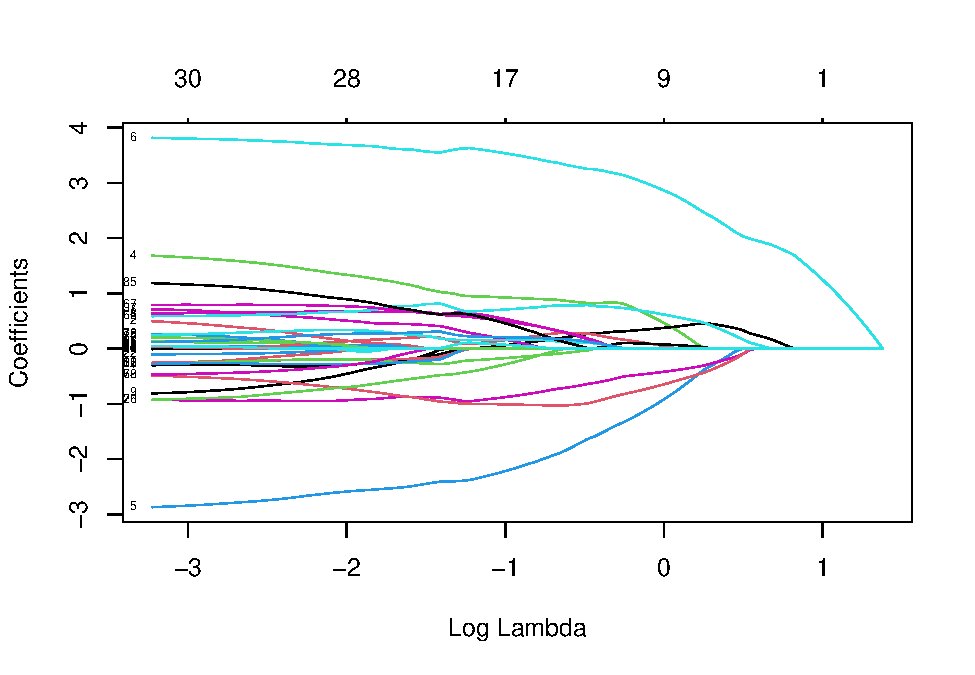
\includegraphics{High-Dimensional-Data-assignments_files/figure-latex/unnamed-chunk-5-1.pdf}

Using the function \texttt{cv.glmnet}, we can find the value of the cross-validated tuning parameter \(\lambda\).

\begin{Shaded}
\begin{Highlighting}[]
\NormalTok{cv_fit_lasso =}\StringTok{ }\KeywordTok{cv.glmnet}\NormalTok{(X, Y)}
\end{Highlighting}
\end{Shaded}

We can visually inspect the mean-squared error for different values of lambda; the two bars along the mean-squared error curve are the upper and the lower standard deviation curves.

\begin{Shaded}
\begin{Highlighting}[]
\KeywordTok{plot}\NormalTok{(cv_fit_lasso)}
\end{Highlighting}
\end{Shaded}

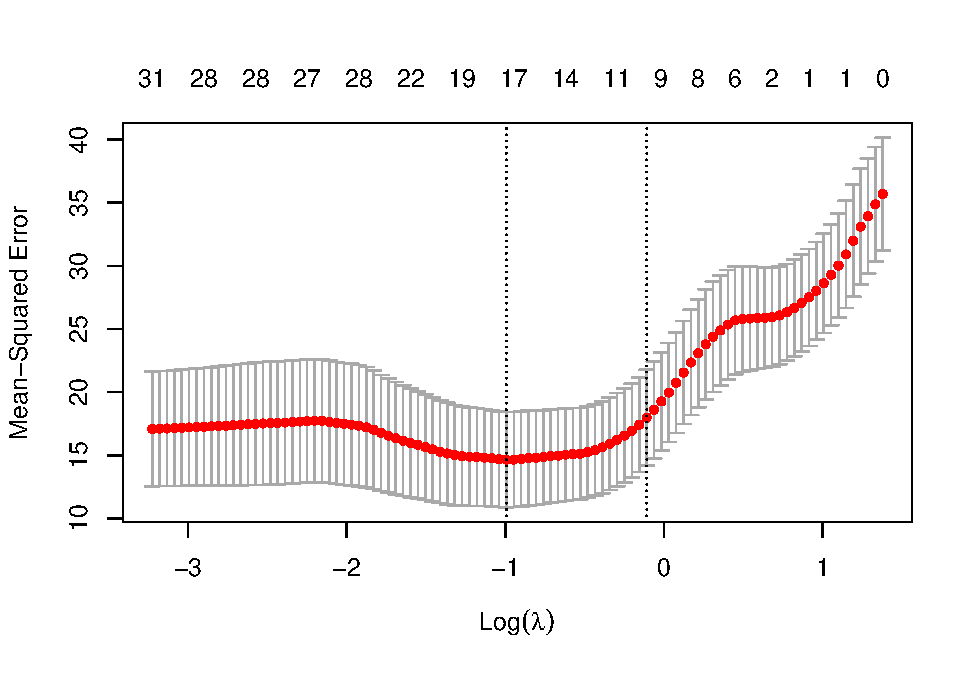
\includegraphics{High-Dimensional-Data-assignments_files/figure-latex/unnamed-chunk-7-1.pdf}

In the plot above, we note that two specific \(\lambda\) values are marked by vertical dotted lines. One of them, denoted by \texttt{lambda.min}, is the value of \(\lambda\) which corresponds to the minimum cross-validated error. The other one, denoted by \texttt{lambda.1se}, is the largest value of \(\lambda\) such that the corresponding cross-validated error is within one standard error of the minimum. This value of \(\lambda\) corresponds to the \emph{most regularized model} with the cross-validated error being within one standard error of the minimum cross-validated error. In case of the lasso, since with increasing \(\lambda\) the number of non-zero coefficients decreases, the number of non-zero coefficients corresponding to \texttt{lambda.1se} is typically lower than that corresponding to \texttt{lambda.min}.

We can access the lambda value corresponding to the minimum cross-validated error in the following way.

\begin{Shaded}
\begin{Highlighting}[]
\NormalTok{lambda_min_lasso =}\StringTok{ }\NormalTok{cv_fit_lasso}\OperatorTok{$}\NormalTok{lambda.min}
\KeywordTok{writeLines}\NormalTok{(}\KeywordTok{paste}\NormalTok{(}\StringTok{'Cross-validated lambda for lasso:'}\NormalTok{,}
\NormalTok{                 lambda_min_lasso))}
\end{Highlighting}
\end{Shaded}

\begin{verbatim}
## Cross-validated lambda for lasso: 0.370549315212255
\end{verbatim}

We can get the coefficients of the fitted model at the cross-validated lambda in the following way.

\begin{Shaded}
\begin{Highlighting}[]
\NormalTok{coefficients_lasso =}\StringTok{ }\KeywordTok{coef}\NormalTok{(cv_fit_lasso, }\DataTypeTok{s =} \StringTok{'lambda.min'}\NormalTok{)}
\KeywordTok{print}\NormalTok{(coefficients_lasso)}
\end{Highlighting}
\end{Shaded}

\begin{verbatim}
## 101 x 1 sparse Matrix of class "dgCMatrix"
##                       1
## (Intercept)  1.80973757
## V1           .         
## V2           .         
## V3           .         
## V4           0.92449282
## V5          -2.21218789
## V6           3.53342728
## V7           .         
## V8           0.53117420
## V9           .         
## V10          .         
## V11          .         
## V12          .         
## V13          .         
## V14          .         
## V15          .         
## V16          .         
## V17          .         
## V18          .         
## V19          .         
## V20          .         
## V21          .         
## V22          .         
## V23          .         
## V24          .         
## V25          .         
## V26         -0.87597982
## V27          0.06242635
## V28          .         
## V29          .         
## V30          .         
## V31          .         
## V32         -0.17019138
## V33          .         
## V34          .         
## V35          .         
## V36          .         
## V37          0.16030531
## V38          .         
## V39          .         
## V40          .         
## V41          .         
## V42          .         
## V43          .         
## V44          .         
## V45          .         
## V46          .         
## V47          0.15672602
## V48          .         
## V49          .         
## V50          .         
## V51          .         
## V52          .         
## V53          .         
## V54          .         
## V55          .         
## V56          .         
## V57          .         
## V58          .         
## V59          .         
## V60          .         
## V61          .         
## V62          .         
## V63          .         
## V64          .         
## V65          0.70974838
## V66          .         
## V67          0.49131462
## V68          .         
## V69         -1.01075761
## V70         -0.27985153
## V71          .         
## V72          .         
## V73          .         
## V74          .         
## V75          0.15711661
## V76          .         
## V77          .         
## V78          .         
## V79          .         
## V80          .         
## V81          .         
## V82          .         
## V83          .         
## V84          .         
## V85          0.45198207
## V86          .         
## V87          .         
## V88          .         
## V89          .         
## V90          .         
## V91          0.20589889
## V92          .         
## V93          .         
## V94          .         
## V95          .         
## V96          .         
## V97          .         
## V98          0.06768265
## V99          .         
## V100         .
\end{verbatim}

As can be seen above, the coefficients are returned in a sparse matrix format. We can convert that to the usual numeric format in the following way. Remember that the intercept term will occupy the first position in the resulting vector.

\begin{Shaded}
\begin{Highlighting}[]
\NormalTok{coefficients_lasso =}\StringTok{ }\KeywordTok{as.numeric}\NormalTok{(coefficients_lasso)}

\CommentTok{# Finding the number of zero coefficients}
\NormalTok{number_zero_coefficients_lasso =}\StringTok{ }\KeywordTok{sum}\NormalTok{(coefficients_lasso }\OperatorTok{==}\StringTok{ }\DecValTok{0}\NormalTok{)}
\KeywordTok{writeLines}\NormalTok{(}\KeywordTok{paste}\NormalTok{(}\StringTok{'Number of zero coefficients in lasso for'}\NormalTok{,}
                 \StringTok{'cross-validated lambda:}\CharTok{\textbackslash{}n}\StringTok{'}\NormalTok{,}
\NormalTok{                 number_zero_coefficients_lasso))}
\end{Highlighting}
\end{Shaded}

\begin{verbatim}
## Number of zero coefficients in lasso for cross-validated lambda:
##  83
\end{verbatim}

\begin{Shaded}
\begin{Highlighting}[]
\CommentTok{# Finding which covariates have a non-zero coefficient in the}
\CommentTok{# fitted model; the '-1' accounts for the intercept term}
\NormalTok{indices_nonzero_coefficients_lasso =}
\StringTok{  }\KeywordTok{which}\NormalTok{(coefficients_lasso }\OperatorTok{!=}\StringTok{ }\DecValTok{0}\NormalTok{) }\OperatorTok{-}\StringTok{ }\DecValTok{1}
\end{Highlighting}
\end{Shaded}

To get the coefficients at the value of \(\lambda\) which gives the most regularized model such that the cross-validated error is within one standard error of the minimum, we use the following command.

\begin{Shaded}
\begin{Highlighting}[]
\NormalTok{coefficients_lasso_most_regularized =}
\StringTok{  }\KeywordTok{coef}\NormalTok{(cv_fit_lasso, }\DataTypeTok{s =} \StringTok{'lambda.1se'}\NormalTok{)}
\NormalTok{coefficients_lasso_most_regularized =}
\StringTok{  }\KeywordTok{as.numeric}\NormalTok{(coefficients_lasso_most_regularized)}

\CommentTok{# Finding the number of zero coefficients}
\NormalTok{number_zero_coefficients_lasso_most_regularized =}
\StringTok{  }\KeywordTok{sum}\NormalTok{(coefficients_lasso_most_regularized }\OperatorTok{==}\StringTok{ }\DecValTok{0}\NormalTok{)}
\KeywordTok{writeLines}\NormalTok{(}\KeywordTok{paste}\NormalTok{(}\StringTok{'Number of zero coefficients in lasso for }\CharTok{\textbackslash{}n}\StringTok{'}\NormalTok{,}
                 \StringTok{'the most regularized model:'}\NormalTok{,}
\NormalTok{                 number_zero_coefficients_lasso_most_regularized))}
\end{Highlighting}
\end{Shaded}

\begin{verbatim}
## Number of zero coefficients in lasso for 
##  the most regularized model: 91
\end{verbatim}

Note that the number of zero coefficients corresponding to \texttt{lambda.1se} is higher than that corresponding to \texttt{lambda.min}. We can find the coefficients at some other value of lambda also, in the same way.

\begin{Shaded}
\begin{Highlighting}[]
\NormalTok{coefficients_lasso_s =}\StringTok{ }\KeywordTok{coef}\NormalTok{(cv_fit_lasso, }\DataTypeTok{s =} \FloatTok{0.5}\NormalTok{)}
\KeywordTok{print}\NormalTok{(coefficients_lasso_s)}
\end{Highlighting}
\end{Shaded}

\begin{verbatim}
## 101 x 1 sparse Matrix of class "dgCMatrix"
##                        1
## (Intercept)  1.767178719
## V1           .          
## V2           .          
## V3           .          
## V4           0.886211639
## V5          -1.930076220
## V6           3.373783767
## V7           .          
## V8           0.337440156
## V9           .          
## V10          .          
## V11          .          
## V12          .          
## V13          .          
## V14          .          
## V15          .          
## V16          .          
## V17          .          
## V18          .          
## V19          .          
## V20          .          
## V21          .          
## V22          .          
## V23          .          
## V24          .          
## V25          .          
## V26         -0.739860240
## V27          0.173458826
## V28          .          
## V29          .          
## V30          .          
## V31          .          
## V32         -0.099445511
## V33          .          
## V34          .          
## V35          .          
## V36          .          
## V37          .          
## V38          .          
## V39          .          
## V40          .          
## V41          .          
## V42          .          
## V43          .          
## V44          .          
## V45          .          
## V46          .          
## V47          0.272255597
## V48          .          
## V49          .          
## V50          .          
## V51          .          
## V52          .          
## V53          .          
## V54          .          
## V55          .          
## V56          .          
## V57          .          
## V58          .          
## V59          .          
## V60          .          
## V61          .          
## V62          .          
## V63          .          
## V64          .          
## V65          0.775881117
## V66          .          
## V67          0.342180469
## V68          .          
## V69         -1.030152116
## V70         -0.049587703
## V71          .          
## V72          .          
## V73          .          
## V74          .          
## V75          0.136389338
## V76          .          
## V77          .          
## V78          .          
## V79          .          
## V80          .          
## V81          .          
## V82          .          
## V83          .          
## V84          .          
## V85          0.173826167
## V86          .          
## V87          .          
## V88          .          
## V89          .          
## V90          .          
## V91          0.178492348
## V92          .          
## V93          .          
## V94          .          
## V95          .          
## V96          .          
## V97          .          
## V98          0.002456585
## V99          .          
## V100         .
\end{verbatim}

To predict the response at some value of the covariates, we use the following command. The argument \texttt{newx} must be supplied as a matrix and not a vector.

\begin{Shaded}
\begin{Highlighting}[]
\NormalTok{x_}\DecValTok{0}\NormalTok{ =}\StringTok{ }\KeywordTok{matrix}\NormalTok{(}\KeywordTok{rnorm}\NormalTok{(}\DecValTok{100}\NormalTok{), }\DataTypeTok{nrow =} \DecValTok{1}\NormalTok{, }\DataTypeTok{ncol =} \DecValTok{100}\NormalTok{)}
\NormalTok{predicted_Y =}\StringTok{ }\KeywordTok{predict}\NormalTok{(cv_fit_lasso, }\DataTypeTok{newx =}\NormalTok{ x_}\DecValTok{0}\NormalTok{, }\DataTypeTok{s =} \StringTok{'lambda.min'}\NormalTok{)}
\KeywordTok{writeLines}\NormalTok{(}\KeywordTok{paste}\NormalTok{(}\StringTok{'Predicted response:'}\NormalTok{, predicted_Y))}
\end{Highlighting}
\end{Shaded}

\begin{verbatim}
## Predicted response: 7.65611533386397
\end{verbatim}

We can predict at several sets of values of the covariates using the same command.

\begin{Shaded}
\begin{Highlighting}[]
\NormalTok{x_}\DecValTok{0}\NormalTok{_values =}\StringTok{ }\KeywordTok{matrix}\NormalTok{(}\KeywordTok{rnorm}\NormalTok{(}\DecValTok{3}\OperatorTok{*}\DecValTok{100}\NormalTok{), }\DataTypeTok{nrow =} \DecValTok{3}\NormalTok{, }\DataTypeTok{ncol =} \DecValTok{100}\NormalTok{)}
\KeywordTok{predict}\NormalTok{(cv_fit_lasso, }\DataTypeTok{newx =}\NormalTok{ x_}\DecValTok{0}\NormalTok{_values, }\DataTypeTok{s =} \StringTok{'lambda.min'}\NormalTok{)}
\end{Highlighting}
\end{Shaded}

\begin{verbatim}
##              1
## [1,]  4.901129
## [2,] -6.576428
## [3,] 10.584152
\end{verbatim}

We can also predict at different values of lambda.

\begin{Shaded}
\begin{Highlighting}[]
\NormalTok{x_}\DecValTok{0}\NormalTok{_values =}\StringTok{ }\KeywordTok{matrix}\NormalTok{(}\KeywordTok{rnorm}\NormalTok{(}\DecValTok{3}\OperatorTok{*}\DecValTok{100}\NormalTok{), }\DataTypeTok{nrow =} \DecValTok{3}\NormalTok{, }\DataTypeTok{ncol =} \DecValTok{100}\NormalTok{)}
\KeywordTok{predict}\NormalTok{(cv_fit_lasso, }\DataTypeTok{newx =}\NormalTok{ x_}\DecValTok{0}\NormalTok{_values, }\DataTypeTok{s =} \KeywordTok{c}\NormalTok{(}\FloatTok{0.5}\NormalTok{, }\FloatTok{0.8}\NormalTok{))}
\end{Highlighting}
\end{Shaded}

\begin{verbatim}
##               1          2
## [1,] -1.3774519 -0.5203943
## [2,]  2.0691667  1.9047106
## [3,] -0.5446435 -0.9182558
\end{verbatim}

\hypertarget{ridge-computation}{%
\subsection{Ridge regression computation}\label{ridge-computation}}

We next demonstrate the ridge regression method. The commands for the ridge regression method are identical with the lasso, except passing the value of another parameter \texttt{alpha\ =\ 0} to the \texttt{glmnet} function, which overwrites the default value of \texttt{alpha\ =\ 1}. The default value \texttt{alpha\ =\ 1} corresponds to the lasso method, and the value \texttt{alpha\ =\ 0} corresponds to ridge regression method.

\begin{Shaded}
\begin{Highlighting}[]
\CommentTok{# Constructing the ridge regression solution paths; 'alpha = 0'}
\CommentTok{# corresponds to the ridge regression method}
\NormalTok{fit_ridge =}\StringTok{ }\KeywordTok{glmnet}\NormalTok{(X, Y, }\DataTypeTok{alpha =} \DecValTok{0}\NormalTok{)}

\CommentTok{# Plotting the ridge regression solution paths}
\KeywordTok{plot}\NormalTok{(fit_ridge, }\DataTypeTok{xvar =} \StringTok{'lambda'}\NormalTok{, }\DataTypeTok{label =} \OtherTok{TRUE}\NormalTok{)}
\end{Highlighting}
\end{Shaded}

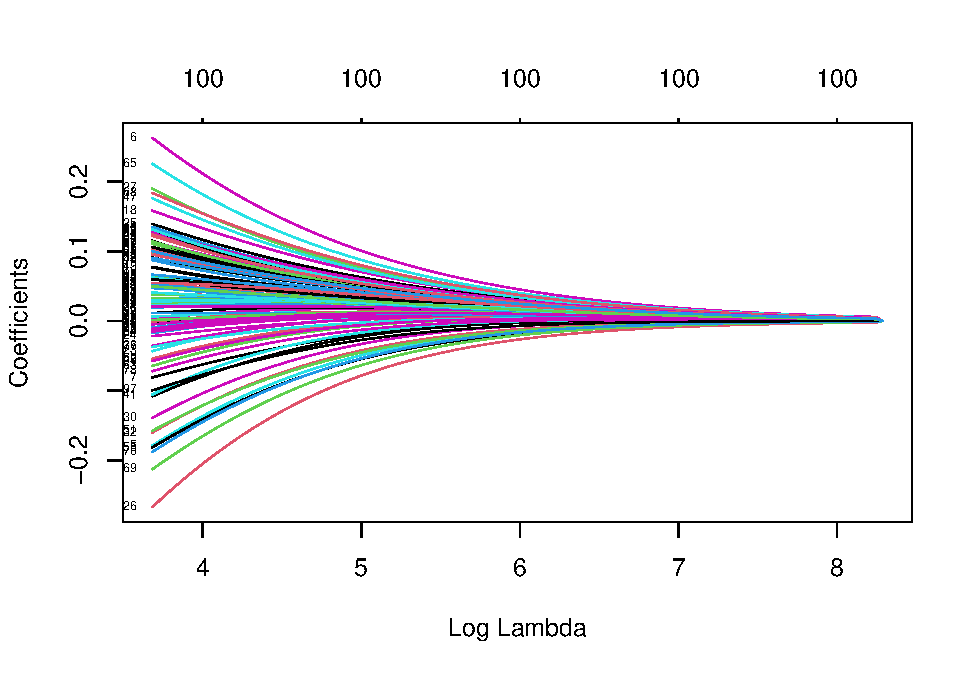
\includegraphics{High-Dimensional-Data-assignments_files/figure-latex/unnamed-chunk-16-1.pdf}

Note that the coefficients do not become zero with inreasing \(\lambda\). The function `cv.glmnet' with \texttt{alpha\ =\ 0} yields the value of the cross-validated \(\lambda\) for the ridge regression.

\begin{Shaded}
\begin{Highlighting}[]
\CommentTok{# 'alpha = 0' corresponds to the ridge regression}
\NormalTok{cv_fit_ridge =}\StringTok{ }\KeywordTok{cv.glmnet}\NormalTok{(X, Y, }\DataTypeTok{alpha =} \DecValTok{0}\NormalTok{)}

\CommentTok{# Plotting the mean-squared error for different values of lambda}
\KeywordTok{plot}\NormalTok{(cv_fit_ridge)}
\end{Highlighting}
\end{Shaded}

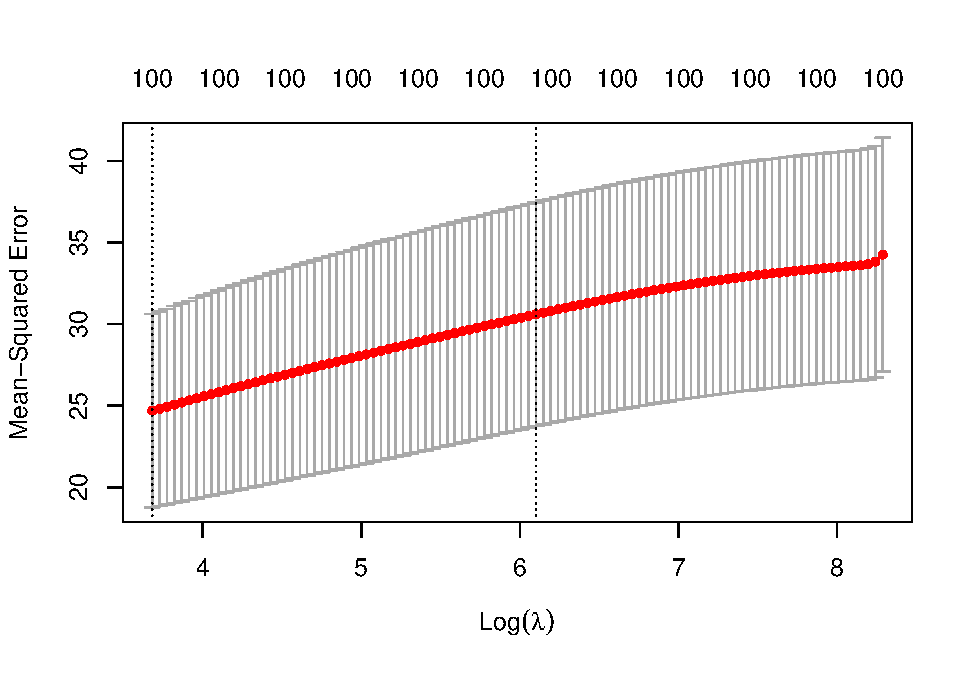
\includegraphics{High-Dimensional-Data-assignments_files/figure-latex/unnamed-chunk-17-1.pdf}

\begin{Shaded}
\begin{Highlighting}[]
\CommentTok{# Accessing the lambda value corresponding to the minimum}
\CommentTok{# cross-validated error}
\NormalTok{lambda_min_ridge =}\StringTok{ }\NormalTok{cv_fit_ridge}\OperatorTok{$}\NormalTok{lambda.min}
\KeywordTok{writeLines}\NormalTok{(}\KeywordTok{paste}\NormalTok{(}\StringTok{'Cross-validated lambda for ridge:'}\NormalTok{,}
\NormalTok{                 lambda_min_ridge))}
\end{Highlighting}
\end{Shaded}

\begin{verbatim}
## Cross-validated lambda for ridge: 39.7327885666703
\end{verbatim}

Below we obtain the coefficients of the fitted ridge regression model at the cross-validated lambda.

\begin{Shaded}
\begin{Highlighting}[]
\NormalTok{coefficients_ridge =}\StringTok{ }\KeywordTok{coef}\NormalTok{(cv_fit_ridge, }\DataTypeTok{s =} \StringTok{'lambda.min'}\NormalTok{)}
\KeywordTok{print}\NormalTok{(coefficients_ridge)}
\end{Highlighting}
\end{Shaded}

\begin{verbatim}
## 101 x 1 sparse Matrix of class "dgCMatrix"
##                         1
## (Intercept)  1.7109491790
## V1          -0.1083085248
## V2           0.0289382846
## V3           0.0874521462
## V4           0.1351638778
## V5          -0.1791263697
## V6           0.2630018834
## V7          -0.0811946853
## V8           0.0953859518
## V9          -0.0567241486
## V10         -0.0092322108
## V11          0.0237973433
## V12          0.0023652437
## V13          0.0627102050
## V14          0.0407541257
## V15          0.0643875969
## V16         -0.0029789548
## V17          0.0239322365
## V18          0.1584882587
## V19          0.0775910313
## V20          0.0384100813
## V21          0.0988288388
## V22         -0.0006264409
## V23         -0.0435152900
## V24         -0.0218175822
## V25          0.1393288850
## V26         -0.2674413045
## V27          0.1901822549
## V28          0.0189121326
## V29          0.0622712797
## V30         -0.1391918705
## V31         -0.0019822390
## V32         -0.1603607166
## V33          0.0386014016
## V34         -0.0175624311
## V35          0.0396806824
## V36         -0.0358246172
## V37          0.0910033959
## V38          0.0600965337
## V39          0.0374900113
## V40          0.0471962575
## V41         -0.1057321976
## V42          0.1279890563
## V43          0.0769178360
## V44          0.0532354797
## V45          0.0255123295
## V46          0.0874539651
## V47          0.1761787139
## V48         -0.0050762765
## V49          0.0596021880
## V50          0.1263894976
## V51         -0.1577883642
## V52         -0.0553016593
## V53          0.0495713021
## V54         -0.0152558775
## V55         -0.1817212663
## V56          0.1037481506
## V57          0.1107477308
## V58          0.0905209790
## V59          0.0279373188
## V60          0.1140120007
## V61          0.1060607717
## V62         -0.0543002730
## V63         -0.0646601361
## V64          0.0535504252
## V65          0.2259343778
## V66         -0.0119965274
## V67          0.1153978110
## V68          0.1839346141
## V69         -0.2130429873
## V70         -0.1881321509
## V71          0.0064749093
## V72          0.1286295451
## V73          0.0595155003
## V74          0.0307595428
## V75          0.1139984619
## V76          0.0322028103
## V77         -0.0374223741
## V78         -0.0721740254
## V79          0.0112816651
## V80         -0.0009252484
## V81          0.0326936742
## V82          0.0665158297
## V83          0.0296031295
## V84          0.0204508045
## V85          0.1315162057
## V86          0.0545900253
## V87          0.0408206632
## V88          0.0112714252
## V89          0.1312721217
## V90         -0.0575812929
## V91          0.1059293353
## V92          0.1223877045
## V93          0.0013630864
## V94          0.0490835634
## V95          0.0408392873
## V96         -0.0113738132
## V97         -0.0997274579
## V98          0.0990380908
## V99          0.0497533756
## V100         0.1000894667
\end{verbatim}

Note that the coefficients are nonzero unlike the lasso. In case of the ridge regression, the value \texttt{lambda.1se} is not so interesting as in case of the lasso, as here there is no question of reducing any coefficient to zero.

\begin{Shaded}
\begin{Highlighting}[]
\NormalTok{coefficients_ridge =}\StringTok{ }\KeywordTok{as.numeric}\NormalTok{(coefficients_ridge)}

\CommentTok{# Finding the number of nonzero coefficients; the '-1' accounts}
\CommentTok{# for the intercept term}
\NormalTok{number_nonzero_coefficients_ridge =}
\StringTok{  }\KeywordTok{sum}\NormalTok{(coefficients_ridge }\OperatorTok{!=}\StringTok{ }\DecValTok{0}\NormalTok{) }\OperatorTok{-}\StringTok{ }\DecValTok{1}
\KeywordTok{writeLines}\NormalTok{(}\KeywordTok{paste}\NormalTok{(}\StringTok{'Number of nonzero coefficients for'}\NormalTok{,}
                 \StringTok{'the ridge regression:}\CharTok{\textbackslash{}n}\StringTok{'}\NormalTok{,}
\NormalTok{                 number_nonzero_coefficients_ridge))}
\end{Highlighting}
\end{Shaded}

\begin{verbatim}
## Number of nonzero coefficients for the ridge regression:
##  100
\end{verbatim}

Finding the coefficients at some other value of lambda is the same as in the case of the lasso.

\begin{Shaded}
\begin{Highlighting}[]
\NormalTok{coefficients_ridge_s =}\StringTok{ }\KeywordTok{coef}\NormalTok{(cv_fit_ridge, }\DataTypeTok{s =} \FloatTok{0.5}\NormalTok{)}
\KeywordTok{print}\NormalTok{(coefficients_ridge_s)}
\end{Highlighting}
\end{Shaded}

\begin{verbatim}
## 101 x 1 sparse Matrix of class "dgCMatrix"
##                         1
## (Intercept)  1.7109491790
## V1          -0.1083085248
## V2           0.0289382846
## V3           0.0874521462
## V4           0.1351638778
## V5          -0.1791263697
## V6           0.2630018834
## V7          -0.0811946853
## V8           0.0953859518
## V9          -0.0567241486
## V10         -0.0092322108
## V11          0.0237973433
## V12          0.0023652437
## V13          0.0627102050
## V14          0.0407541257
## V15          0.0643875969
## V16         -0.0029789548
## V17          0.0239322365
## V18          0.1584882587
## V19          0.0775910313
## V20          0.0384100813
## V21          0.0988288388
## V22         -0.0006264409
## V23         -0.0435152900
## V24         -0.0218175822
## V25          0.1393288850
## V26         -0.2674413045
## V27          0.1901822549
## V28          0.0189121326
## V29          0.0622712797
## V30         -0.1391918705
## V31         -0.0019822390
## V32         -0.1603607166
## V33          0.0386014016
## V34         -0.0175624311
## V35          0.0396806824
## V36         -0.0358246172
## V37          0.0910033959
## V38          0.0600965337
## V39          0.0374900113
## V40          0.0471962575
## V41         -0.1057321976
## V42          0.1279890563
## V43          0.0769178360
## V44          0.0532354797
## V45          0.0255123295
## V46          0.0874539651
## V47          0.1761787139
## V48         -0.0050762765
## V49          0.0596021880
## V50          0.1263894976
## V51         -0.1577883642
## V52         -0.0553016593
## V53          0.0495713021
## V54         -0.0152558775
## V55         -0.1817212663
## V56          0.1037481506
## V57          0.1107477308
## V58          0.0905209790
## V59          0.0279373188
## V60          0.1140120007
## V61          0.1060607717
## V62         -0.0543002730
## V63         -0.0646601361
## V64          0.0535504252
## V65          0.2259343778
## V66         -0.0119965274
## V67          0.1153978110
## V68          0.1839346141
## V69         -0.2130429873
## V70         -0.1881321509
## V71          0.0064749093
## V72          0.1286295451
## V73          0.0595155003
## V74          0.0307595428
## V75          0.1139984619
## V76          0.0322028103
## V77         -0.0374223741
## V78         -0.0721740254
## V79          0.0112816651
## V80         -0.0009252484
## V81          0.0326936742
## V82          0.0665158297
## V83          0.0296031295
## V84          0.0204508045
## V85          0.1315162057
## V86          0.0545900253
## V87          0.0408206632
## V88          0.0112714252
## V89          0.1312721217
## V90         -0.0575812929
## V91          0.1059293353
## V92          0.1223877045
## V93          0.0013630864
## V94          0.0490835634
## V95          0.0408392873
## V96         -0.0113738132
## V97         -0.0997274579
## V98          0.0990380908
## V99          0.0497533756
## V100         0.1000894667
\end{verbatim}

We can also predict at several sets of values of the covariates and at different values of lambda for the fitted ridge regression model. The argument \texttt{newx} always must be a matrix, even if we are predicting at only one set of values of the covariates.

\begin{Shaded}
\begin{Highlighting}[]
\NormalTok{x_}\DecValTok{0}\NormalTok{_values =}\StringTok{ }\KeywordTok{matrix}\NormalTok{(}\KeywordTok{rnorm}\NormalTok{(}\DecValTok{3}\OperatorTok{*}\DecValTok{100}\NormalTok{), }\DataTypeTok{nrow =} \DecValTok{3}\NormalTok{, }\DataTypeTok{ncol =} \DecValTok{100}\NormalTok{)}
\KeywordTok{predict}\NormalTok{(cv_fit_ridge, }\DataTypeTok{newx =}\NormalTok{ x_}\DecValTok{0}\NormalTok{_values, }\DataTypeTok{s =} \KeywordTok{c}\NormalTok{(}\FloatTok{0.5}\NormalTok{, }\FloatTok{0.8}\NormalTok{))}
\end{Highlighting}
\end{Shaded}

\begin{verbatim}
##              1         2
## [1,] 2.2248989 2.2248989
## [2,] 2.5238977 2.5238977
## [3,] 0.3758271 0.3758271
\end{verbatim}

\hypertarget{elasticnet-computation}{%
\subsection{Elastic net computation}\label{elasticnet-computation}}

From the description of the elastic net in subsection \ref{elasticnet-description}, and the codes for computing the lasso and the ridge regression solutions in subsection \ref{lasso-computation} and subsection \ref{ridge-computation} respectively, you might have guessed that the function \texttt{glmnet} actually computed the elastic net solutions for different values of the parameter \(\alpha\): \(\alpha = 1\) corresponds to the lasso and \(\alpha = 0\) corresponds to the ridge regression method. So, the same code with a value of the argument \texttt{alpha} in \((0, 1)\) will return the elastic net solution for that value of \(\alpha\). Below, we demonstrate the computation for \(\alpha = 0.5\).

\begin{Shaded}
\begin{Highlighting}[]
\CommentTok{# Constructing the elastic net solution paths for 'alpha = 0.5'}
\NormalTok{fit_elnet =}\StringTok{ }\KeywordTok{glmnet}\NormalTok{(X, Y, }\DataTypeTok{alpha =} \FloatTok{0.5}\NormalTok{)}

\CommentTok{# Plotting the elastic net solution paths}
\KeywordTok{plot}\NormalTok{(fit_elnet, }\DataTypeTok{xvar =} \StringTok{'lambda'}\NormalTok{, }\DataTypeTok{label =} \OtherTok{TRUE}\NormalTok{)}
\end{Highlighting}
\end{Shaded}

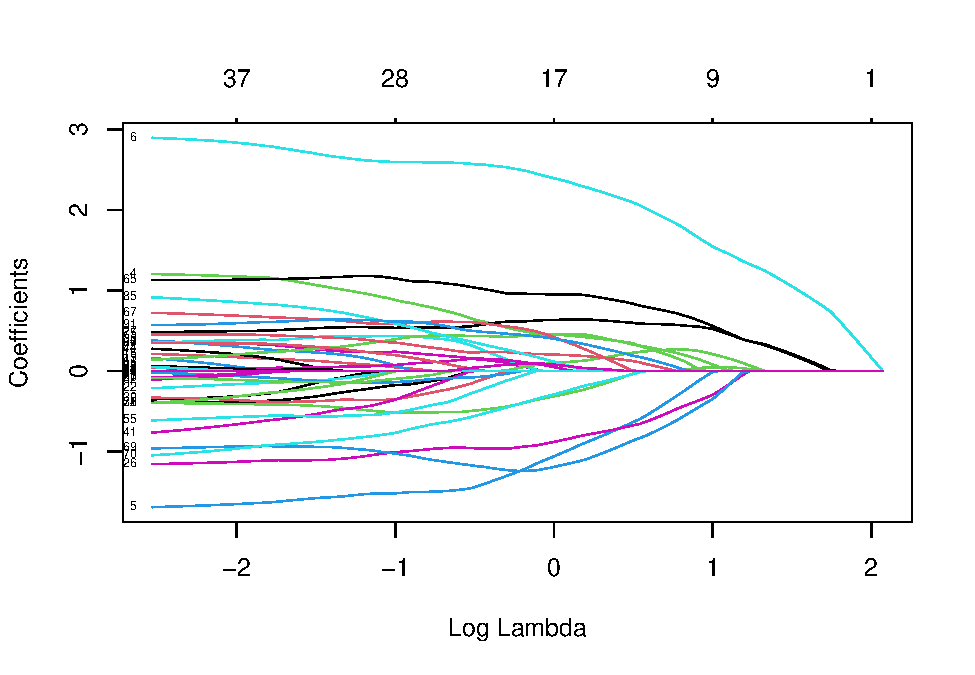
\includegraphics{High-Dimensional-Data-assignments_files/figure-latex/unnamed-chunk-22-1.pdf}

Note that the coefficients become zero with inreasing \(\lambda\) like in the case of the lasso.

\begin{Shaded}
\begin{Highlighting}[]
\CommentTok{# Cross-validation for elastic net with 'alpha = 0.5'}
\NormalTok{cv_fit_elnet =}\StringTok{ }\KeywordTok{cv.glmnet}\NormalTok{(X, Y, }\DataTypeTok{alpha =} \FloatTok{0.5}\NormalTok{)}

\CommentTok{# Plotting the mean-squared error for different values of lambda}
\KeywordTok{plot}\NormalTok{(cv_fit_elnet)}
\end{Highlighting}
\end{Shaded}

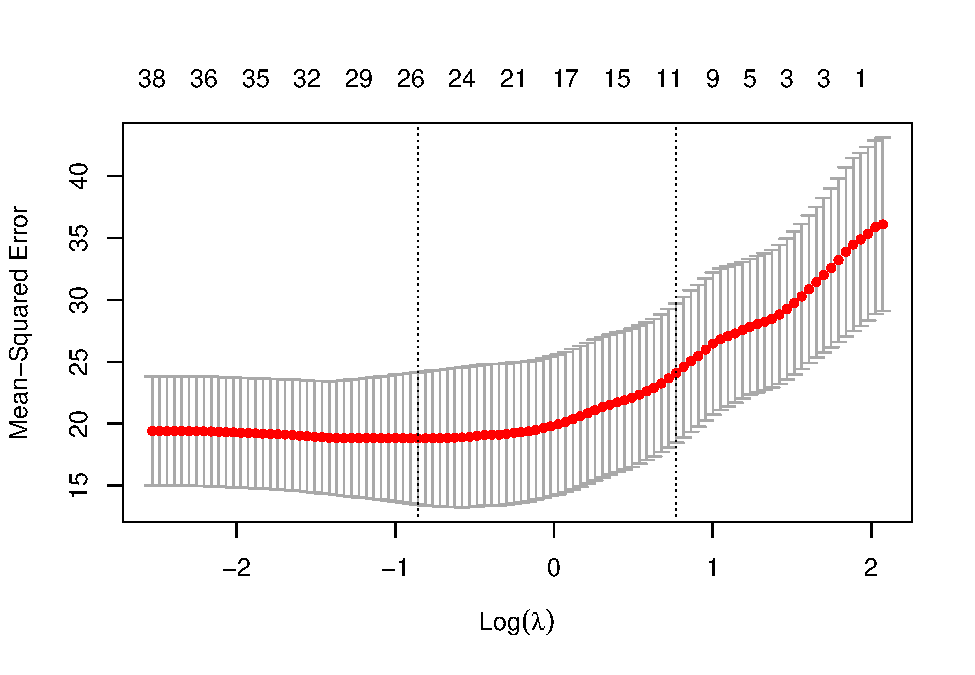
\includegraphics{High-Dimensional-Data-assignments_files/figure-latex/unnamed-chunk-23-1.pdf}

\begin{Shaded}
\begin{Highlighting}[]
\CommentTok{# Accessing the lambda value corresponding to the minimum}
\CommentTok{# cross-validated error}
\NormalTok{lambda_min_elnet =}\StringTok{ }\NormalTok{cv_fit_elnet}\OperatorTok{$}\NormalTok{lambda.min}
\KeywordTok{writeLines}\NormalTok{(}\KeywordTok{paste}\NormalTok{(}\StringTok{'Cross-validated lambda for elastic net:'}\NormalTok{,}
\NormalTok{                 lambda_min_elnet))}
\end{Highlighting}
\end{Shaded}

\begin{verbatim}
## Cross-validated lambda for elastic net: 0.424083883733463
\end{verbatim}

\begin{Shaded}
\begin{Highlighting}[]
\CommentTok{# Coefficients of the fitted elastic net at the cross-validated}
\CommentTok{# lambda}
\NormalTok{coefficients_elnet =}\StringTok{ }\KeywordTok{coef}\NormalTok{(cv_fit_elnet, }\DataTypeTok{s =} \StringTok{'lambda.min'}\NormalTok{)}
\KeywordTok{print}\NormalTok{(coefficients_elnet)}
\end{Highlighting}
\end{Shaded}

\begin{verbatim}
## 101 x 1 sparse Matrix of class "dgCMatrix"
##                       1
## (Intercept)  2.11279990
## V1          -0.15092287
## V2           .         
## V3           .         
## V4           0.82409055
## V5          -1.50317945
## V6           2.59241473
## V7           .         
## V8           0.21545204
## V9           .         
## V10          .         
## V11          .         
## V12          .         
## V13          .         
## V14          .         
## V15          0.02007609
## V16          .         
## V17          .         
## V18          .         
## V19          .         
## V20          .         
## V21          .         
## V22          .         
## V23          .         
## V24          .         
## V25          .         
## V26         -0.98502236
## V27          0.54189086
## V28          .         
## V29          .         
## V30         -0.30190044
## V31          .         
## V32         -0.51413064
## V33          .         
## V34          .         
## V35          .         
## V36          .         
## V37          0.42556645
## V38          .         
## V39          .         
## V40          .         
## V41         -0.25103694
## V42          .         
## V43          .         
## V44          .         
## V45          .         
## V46          .         
## V47          0.42890488
## V48          .         
## V49          .         
## V50          .         
## V51         -0.11850576
## V52          .         
## V53          .         
## V54          .         
## V55         -0.46259584
## V56          .         
## V57          .         
## V58          .         
## V59          .         
## V60          .         
## V61          .         
## V62          .         
## V63          .         
## V64          .         
## V65          1.11118958
## V66          .         
## V67          0.60206411
## V68          .         
## V69         -1.07119524
## V70         -0.70044278
## V71          .         
## V72          0.09785610
## V73          .         
## V74          .         
## V75          0.31266992
## V76          .         
## V77          .         
## V78          .         
## V79          .         
## V80          .         
## V81          .         
## V82          .         
## V83          .         
## V84          .         
## V85          0.51997636
## V86          .         
## V87          .         
## V88          .         
## V89          0.15174385
## V90         -0.07005343
## V91          0.60397991
## V92          .         
## V93          .         
## V94          .         
## V95          .         
## V96          .         
## V97          .         
## V98          .         
## V99          .         
## V100         .
\end{verbatim}

Note that many of the coefficients are zero like the lasso. However, the number of zero coefficients is lower than the lasso.

\begin{Shaded}
\begin{Highlighting}[]
\NormalTok{coefficients_elnet =}\StringTok{ }\KeywordTok{as.numeric}\NormalTok{(coefficients_elnet)}

\CommentTok{# Finding the number of nonzero coefficients; the '-1' accounts}
\CommentTok{# for the intercept term}
\NormalTok{number_nonzero_coefficients_elnet =}
\StringTok{  }\KeywordTok{sum}\NormalTok{(coefficients_elnet }\OperatorTok{!=}\StringTok{ }\DecValTok{0}\NormalTok{) }\OperatorTok{-}\StringTok{ }\DecValTok{1}
\KeywordTok{writeLines}\NormalTok{(}\KeywordTok{paste}\NormalTok{(}\StringTok{'Number of nonzero coefficients for'}\NormalTok{,}
                 \StringTok{'the elastic net:'}\NormalTok{,}
\NormalTok{                 number_nonzero_coefficients_elnet))}
\end{Highlighting}
\end{Shaded}

\begin{verbatim}
## Number of nonzero coefficients for the elastic net: 25
\end{verbatim}

\begin{Shaded}
\begin{Highlighting}[]
\CommentTok{# Computing the coefficients at some other value of lambda}
\NormalTok{coefficients_elnet_s =}\StringTok{ }\KeywordTok{coef}\NormalTok{(cv_fit_elnet, }\DataTypeTok{s =} \FloatTok{0.5}\NormalTok{)}
\KeywordTok{print}\NormalTok{(coefficients_elnet_s)}
\end{Highlighting}
\end{Shaded}

\begin{verbatim}
## 101 x 1 sparse Matrix of class "dgCMatrix"
##                       1
## (Intercept)  2.04051028
## V1          -0.09756072
## V2           .         
## V3           .         
## V4           0.75068788
## V5          -1.49223014
## V6           2.58752206
## V7           .         
## V8           0.18902712
## V9           .         
## V10          .         
## V11          .         
## V12          .         
## V13          .         
## V14          .         
## V15          .         
## V16          .         
## V17          .         
## V18          .         
## V19          .         
## V20          .         
## V21          .         
## V22          .         
## V23          .         
## V24          .         
## V25          .         
## V26         -0.95807495
## V27          0.53735119
## V28          .         
## V29          .         
## V30         -0.23907252
## V31          .         
## V32         -0.51110747
## V33          .         
## V34          .         
## V35          .         
## V36          .         
## V37          0.39406628
## V38          .         
## V39          .         
## V40          .         
## V41         -0.12997961
## V42          .         
## V43          .         
## V44          .         
## V45          .         
## V46          .         
## V47          0.44055872
## V48          .         
## V49          .         
## V50          .         
## V51         -0.09072844
## V52          .         
## V53          .         
## V54          .         
## V55         -0.39664432
## V56          .         
## V57          .         
## V58          .         
## V59          .         
## V60          .         
## V61          .         
## V62          .         
## V63          .         
## V64          .         
## V65          1.08905420
## V66          .         
## V67          0.61168096
## V68          .         
## V69         -1.12571292
## V70         -0.63958967
## V71          .         
## V72          0.11705065
## V73          .         
## V74          .         
## V75          0.27052397
## V76          .         
## V77          .         
## V78          .         
## V79          .         
## V80          .         
## V81          .         
## V82          .         
## V83          .         
## V84          .         
## V85          0.43965564
## V86          .         
## V87          .         
## V88          .         
## V89          0.09232706
## V90         -0.01848038
## V91          0.56203662
## V92          .         
## V93          .         
## V94          .         
## V95          .         
## V96          .         
## V97          .         
## V98          .         
## V99          .         
## V100         .
\end{verbatim}

\begin{Shaded}
\begin{Highlighting}[]
\CommentTok{# Predicting at several sets of values of the covariates and at}
\CommentTok{# different values of lambda for the fitted elastic net}
\NormalTok{x_}\DecValTok{0}\NormalTok{_values =}\StringTok{ }\KeywordTok{matrix}\NormalTok{(}\KeywordTok{rnorm}\NormalTok{(}\DecValTok{3}\OperatorTok{*}\DecValTok{100}\NormalTok{), }\DataTypeTok{nrow =} \DecValTok{3}\NormalTok{, }\DataTypeTok{ncol =} \DecValTok{100}\NormalTok{)}
\KeywordTok{predict}\NormalTok{(cv_fit_elnet, }\DataTypeTok{newx =}\NormalTok{ x_}\DecValTok{0}\NormalTok{_values, }\DataTypeTok{s =} \KeywordTok{c}\NormalTok{(}\FloatTok{0.5}\NormalTok{, }\FloatTok{0.8}\NormalTok{))}
\end{Highlighting}
\end{Shaded}

\begin{verbatim}
##              1         2
## [1,] -6.386536 -4.828346
## [2,]  3.403320  2.583454
## [3,] -3.042642 -3.058112
\end{verbatim}

\hypertarget{adaptivelasso-computation}{%
\subsection{Adaptive lasso computation}\label{adaptivelasso-computation}}

Recall the description of the adaptive lasso method in subsection \ref{adaptivelasso-description}. We shall demonstrate the adaptive lasso with \(\gamma = 1\) taking the usual cross-validated lasso solution as the initial estimate.

First we compute the cross-validated lasso solution.

\begin{Shaded}
\begin{Highlighting}[]
\CommentTok{# Computing the coefficient for the cross-validated lasso estimate}
\NormalTok{cv_fit_lasso =}\StringTok{ }\KeywordTok{cv.glmnet}\NormalTok{(X, Y)}
\NormalTok{coefficients_lasso =}\StringTok{ }\KeywordTok{coef}\NormalTok{(cv_fit_lasso, }\DataTypeTok{s =} \StringTok{'lambda.min'}\NormalTok{)}

\CommentTok{# Dropping the intercept term in the cross-validated lasso}
\CommentTok{# estimate}
\NormalTok{coefficients_lasso =}\StringTok{ }\KeywordTok{as.numeric}\NormalTok{(coefficients_lasso)[}\OperatorTok{-}\DecValTok{1}\NormalTok{]}

\CommentTok{# Computing the adaptive lasso estimate. The argument}
\CommentTok{# 'penalty.factor' assigns weights to the coefficients, with the}
\CommentTok{# convention of r / 0 = Infinity for r > 0.}
\NormalTok{cv_fit_adaptive =}
\StringTok{  }\KeywordTok{cv.glmnet}\NormalTok{(X, Y, }\DataTypeTok{penalty.factor =} \DecValTok{1} \OperatorTok{/}\StringTok{ }\KeywordTok{abs}\NormalTok{(coefficients_lasso))}
\NormalTok{coefficients_adaptive =}\StringTok{ }\KeywordTok{coef}\NormalTok{(cv_fit_adaptive, }\DataTypeTok{s =} \StringTok{'lambda.min'}\NormalTok{)}

\CommentTok{# Dropping the intercept term for the adaptive lasso estimate}
\NormalTok{coefficients_adaptive =}\StringTok{ }\KeywordTok{as.numeric}\NormalTok{(coefficients_adaptive)[}\OperatorTok{-}\DecValTok{1}\NormalTok{]}
\end{Highlighting}
\end{Shaded}

Recall from subsection \ref{adaptivelasso-description} that the adaptive lasso estimate is sparser than the lasso estimate. From the construction of our simulation setup, we know that only the coefficients of \(X_1\), \(X_2\), \(X_3\), \(X_4\), \(X_5\) and \(X_6\) are nonzero in the underlying model. Let us see the indices of the covariates with nonzero coefficients in the lasso estimate and the adaptive lasso estimate.

\begin{Shaded}
\begin{Highlighting}[]
\KeywordTok{writeLines}\NormalTok{(}\KeywordTok{paste}\NormalTok{(}\StringTok{'Indices of the covariates with nonzero'}\NormalTok{,}
                 \StringTok{'coefficients }\CharTok{\textbackslash{}n}\StringTok{ for the lasso estimate:}\CharTok{\textbackslash{}n}\StringTok{'}\NormalTok{,}
                 \KeywordTok{paste}\NormalTok{(}\KeywordTok{which}\NormalTok{(coefficients_lasso }\OperatorTok{!=}\StringTok{ }\DecValTok{0}\NormalTok{),}
                       \DataTypeTok{collapse =} \StringTok{' '}\NormalTok{)))}
\end{Highlighting}
\end{Shaded}

\begin{verbatim}
## Indices of the covariates with nonzero coefficients 
##  for the lasso estimate:
##  4 5 6 8 26 27 32 37 47 65 67 69 70 75 85 91 98
\end{verbatim}

\begin{Shaded}
\begin{Highlighting}[]
\KeywordTok{writeLines}\NormalTok{(}\KeywordTok{paste}\NormalTok{(}\StringTok{'Indices of the covariates with nonzero'}\NormalTok{,}
                 \StringTok{'coefficients }\CharTok{\textbackslash{}n}\StringTok{ for the adaptive lasso'}\NormalTok{,}
                 \StringTok{'estimate:}\CharTok{\textbackslash{}n}\StringTok{'}\NormalTok{,}
                 \KeywordTok{paste}\NormalTok{(}\KeywordTok{which}\NormalTok{(coefficients_adaptive }\OperatorTok{!=}\StringTok{ }\DecValTok{0}\NormalTok{),}
                       \DataTypeTok{collapse =} \StringTok{' '}\NormalTok{)))}
\end{Highlighting}
\end{Shaded}

\begin{verbatim}
## Indices of the covariates with nonzero coefficients 
##  for the adaptive lasso estimate:
##  4 5 6 8 26 65 67 69 85
\end{verbatim}

We note that the lasso estimate has 17 nonzero coordinates, while the adaptive lasso has 9 nonzero coordinates. So, the adaptive lasso estimate is indeed sparser than the lasso estimate. However, both of them erroneously estimate several zero coefficients as nonzero, and fail to capture several nonzero coefficients.

\hypertarget{grouplasso-computation}{%
\subsection{Group lasso computation}\label{grouplasso-computation}}

For the group lasso computation, we shall use the \texttt{gglasso} package by \citet{R-gglasso}. We shall use the same simulation setup, but the covariates will be divided in groups in the following way: \(X_1, \ldots, X_5\) in the first group, \(X_6, \ldots, X_10\) in the second group, and so on. We form the group indices below, which will be required.

\begin{Shaded}
\begin{Highlighting}[]
\NormalTok{group_indices =}\StringTok{ }\KeywordTok{c}\NormalTok{()}
\ControlFlowTok{for}\NormalTok{ (i }\ControlFlowTok{in} \DecValTok{1}\OperatorTok{:}\DecValTok{20}\NormalTok{)}
\NormalTok{  group_indices =}\StringTok{ }\KeywordTok{c}\NormalTok{(group_indices, }\KeywordTok{rep}\NormalTok{(i, }\DecValTok{5}\NormalTok{))}
\KeywordTok{writeLines}\NormalTok{(}\StringTok{'First 20 group indices are:'}\NormalTok{)}
\end{Highlighting}
\end{Shaded}

\begin{verbatim}
## First 20 group indices are:
\end{verbatim}

\begin{Shaded}
\begin{Highlighting}[]
\KeywordTok{print}\NormalTok{(group_indices[}\DecValTok{1}\OperatorTok{:}\DecValTok{20}\NormalTok{])}
\end{Highlighting}
\end{Shaded}

\begin{verbatim}
##  [1] 1 1 1 1 1 2 2 2 2 2 3 3 3 3 3 4 4 4 4 4
\end{verbatim}

The following command installs the package \texttt{gglasso}.

\begin{Shaded}
\begin{Highlighting}[]
\KeywordTok{install.packages}\NormalTok{(}\StringTok{'gglasso'}\NormalTok{)}
\end{Highlighting}
\end{Shaded}

We now demonstrate the computation for the group lasso method. The commands are very similar to those in \texttt{glmnet}.

\begin{Shaded}
\begin{Highlighting}[]
\CommentTok{# Loading the 'gglasso' package}
\KeywordTok{require}\NormalTok{(gglasso)}

\CommentTok{# Constructing the group lasso solution paths}
\NormalTok{fit_group =}\StringTok{ }\KeywordTok{gglasso}\NormalTok{(X, Y, }\DataTypeTok{group =}\NormalTok{ group_indices)}

\CommentTok{# Plotting the ridge regression solution paths; the}
\CommentTok{# 'label' argument does not work here, unfortunately.}
\KeywordTok{plot}\NormalTok{(fit_group, }\DataTypeTok{xvar =} \StringTok{'lambda'}\NormalTok{)}
\end{Highlighting}
\end{Shaded}

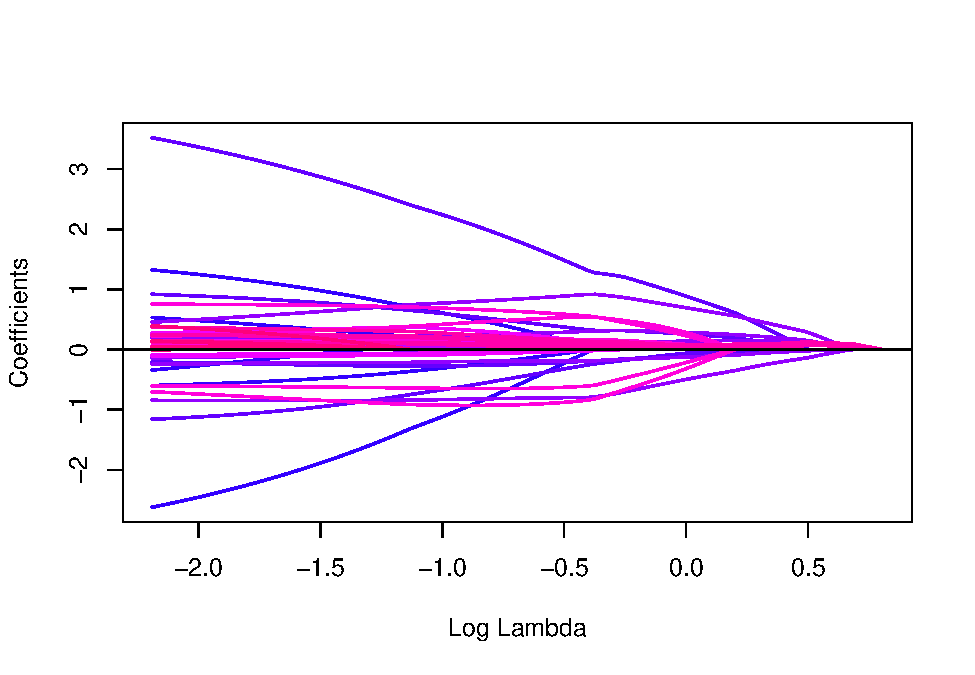
\includegraphics{High-Dimensional-Data-assignments_files/figure-latex/unnamed-chunk-29-1.pdf}

\begin{Shaded}
\begin{Highlighting}[]
\CommentTok{# Cross-validation for group lasso; 'nfolds' is a}
\CommentTok{# cross-validation parameter whose default value}
\CommentTok{# was 10 in our earlier calculations using the 'glmnet'}
\CommentTok{# package. Since its default parameter for the 'gglasso'}
\CommentTok{# package is different, we set that explicitly to 10}
\CommentTok{# here to maintain uniformity.}
\NormalTok{cv_fit_group =}\StringTok{ }\KeywordTok{cv.gglasso}\NormalTok{(X, Y, }\DataTypeTok{group =}\NormalTok{ group_indices,}
                          \DataTypeTok{nfolds =} \DecValTok{10}\NormalTok{)}

\CommentTok{# Plotting the mean-squared error for different values of}
\CommentTok{# lambda in the group lasso cross-validation}
\KeywordTok{plot}\NormalTok{(cv_fit_group)}
\end{Highlighting}
\end{Shaded}

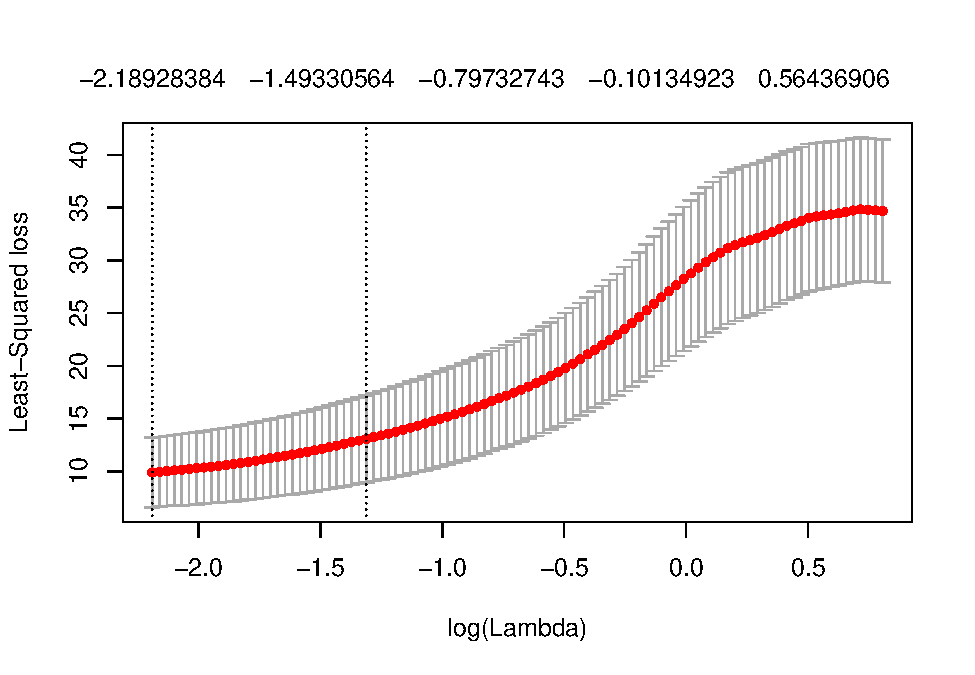
\includegraphics{High-Dimensional-Data-assignments_files/figure-latex/unnamed-chunk-29-2.pdf}

\begin{Shaded}
\begin{Highlighting}[]
\CommentTok{# Getting the lambda value corresponding to the minimum}
\CommentTok{# cross-validated error in the group lasso}
\NormalTok{lambda_min_group =}\StringTok{ }\NormalTok{cv_fit_group}\OperatorTok{$}\NormalTok{lambda.min}
\KeywordTok{writeLines}\NormalTok{(}\KeywordTok{paste}\NormalTok{(}\StringTok{'Cross-validated lambda for group lasso:'}\NormalTok{,}
\NormalTok{                 lambda_min_group))}
\end{Highlighting}
\end{Shaded}

\begin{verbatim}
## Cross-validated lambda for group lasso: 0.111996927450172
\end{verbatim}

\begin{Shaded}
\begin{Highlighting}[]
\CommentTok{# Coefficients of the fitted group lasso at the}
\CommentTok{# cross-validated lambda}
\NormalTok{coefficients_group =}\StringTok{ }\KeywordTok{coef}\NormalTok{(cv_fit_group, }\DataTypeTok{s =} \StringTok{'lambda.min'}\NormalTok{)}
\KeywordTok{print}\NormalTok{(coefficients_group)}
\end{Highlighting}
\end{Shaded}

\begin{verbatim}
##                        1
## (Intercept)  2.299964945
## V1          -0.597276460
## V2           0.532650084
## V3          -0.341296086
## V4           1.324008186
## V5          -2.620777857
## V6           3.520635169
## V7          -0.205739578
## V8           0.919717629
## V9          -1.158546608
## V10         -0.115243566
## V11          0.000000000
## V12          0.000000000
## V13          0.000000000
## V14          0.000000000
## V15          0.000000000
## V16          0.000000000
## V17          0.000000000
## V18          0.000000000
## V19          0.000000000
## V20          0.000000000
## V21          0.000000000
## V22          0.000000000
## V23          0.000000000
## V24          0.000000000
## V25          0.000000000
## V26         -0.843269703
## V27          0.454718935
## V28         -0.139688699
## V29          0.198558378
## V30         -0.245208698
## V31          0.000000000
## V32          0.000000000
## V33          0.000000000
## V34          0.000000000
## V35          0.000000000
## V36          0.000000000
## V37          0.000000000
## V38          0.000000000
## V39          0.000000000
## V40          0.000000000
## V41          0.000000000
## V42          0.000000000
## V43          0.000000000
## V44          0.000000000
## V45          0.000000000
## V46          0.049197887
## V47          0.133784587
## V48          0.006353655
## V49          0.000623473
## V50          0.051280996
## V51          0.000000000
## V52          0.000000000
## V53          0.000000000
## V54          0.000000000
## V55          0.000000000
## V56          0.000000000
## V57          0.000000000
## V58          0.000000000
## V59          0.000000000
## V60          0.000000000
## V61          0.127846059
## V62         -0.102298726
## V63         -0.084174083
## V64          0.140865202
## V65          0.276307972
## V66          0.055334287
## V67          0.754238086
## V68          0.215257426
## V69         -0.700822526
## V70         -0.602696078
## V71          0.147769008
## V72          0.245420916
## V73          0.242587489
## V74          0.126254804
## V75          0.371727647
## V76          0.000000000
## V77          0.000000000
## V78          0.000000000
## V79          0.000000000
## V80          0.000000000
## V81          0.048401665
## V82         -0.008353210
## V83          0.140023712
## V84          0.139982310
## V85          0.392935904
## V86          0.000000000
## V87          0.000000000
## V88          0.000000000
## V89          0.000000000
## V90          0.000000000
## V91          0.000000000
## V92          0.000000000
## V93          0.000000000
## V94          0.000000000
## V95          0.000000000
## V96          0.000000000
## V97          0.000000000
## V98          0.000000000
## V99          0.000000000
## V100         0.000000000
\end{verbatim}

\begin{Shaded}
\begin{Highlighting}[]
\CommentTok{# Computing the coefficients at some other value of lambda}
\CommentTok{# for the group lasso estimate}
\NormalTok{coefficients_group_s =}\StringTok{ }\KeywordTok{coef}\NormalTok{(cv_fit_group, }\DataTypeTok{s =} \FloatTok{0.5}\NormalTok{)}
\KeywordTok{print}\NormalTok{(coefficients_group_s)}
\end{Highlighting}
\end{Shaded}

\begin{verbatim}
##                        1
## (Intercept)  2.446545801
## V1          -0.164606301
## V2           0.094789057
## V3           0.120037112
## V4           0.347808507
## V5          -0.593803459
## V6           1.804429746
## V7          -0.246614547
## V8           0.464199928
## V9          -0.460855429
## V10          0.019794050
## V11          0.000000000
## V12          0.000000000
## V13          0.000000000
## V14          0.000000000
## V15          0.000000000
## V16          0.000000000
## V17          0.000000000
## V18          0.000000000
## V19          0.000000000
## V20          0.000000000
## V21          0.000000000
## V22          0.000000000
## V23          0.000000000
## V24          0.000000000
## V25          0.000000000
## V26         -0.810113871
## V27          0.839345222
## V28          0.008647552
## V29          0.261184248
## V30         -0.190066878
## V31          0.000000000
## V32          0.000000000
## V33          0.000000000
## V34          0.000000000
## V35          0.000000000
## V36          0.000000000
## V37          0.000000000
## V38          0.000000000
## V39          0.000000000
## V40          0.000000000
## V41          0.000000000
## V42          0.000000000
## V43          0.000000000
## V44          0.000000000
## V45          0.000000000
## V46          0.007239078
## V47          0.015033387
## V48          0.003418754
## V49          0.004555346
## V50          0.010936767
## V51          0.000000000
## V52          0.000000000
## V53          0.000000000
## V54          0.000000000
## V55          0.000000000
## V56          0.000000000
## V57          0.000000000
## V58          0.000000000
## V59          0.000000000
## V60          0.000000000
## V61          0.131674540
## V62         -0.054091098
## V63         -0.033632054
## V64          0.092040935
## V65          0.258461382
## V66          0.172478602
## V67          0.634772294
## V68          0.494381080
## V69         -0.917556135
## V70         -0.647221136
## V71          0.053041142
## V72          0.137248090
## V73          0.147020100
## V74          0.094450596
## V75          0.202158872
## V76          0.000000000
## V77          0.000000000
## V78          0.000000000
## V79          0.000000000
## V80          0.000000000
## V81          0.000000000
## V82          0.000000000
## V83          0.000000000
## V84          0.000000000
## V85          0.000000000
## V86          0.000000000
## V87          0.000000000
## V88          0.000000000
## V89          0.000000000
## V90          0.000000000
## V91          0.000000000
## V92          0.000000000
## V93          0.000000000
## V94          0.000000000
## V95          0.000000000
## V96          0.000000000
## V97          0.000000000
## V98          0.000000000
## V99          0.000000000
## V100         0.000000000
\end{verbatim}

Notice that the group lasso method reduces to zero all the coefficients together in any group. Next, we predict the group lasso estimate at some sets of values of the covariates.

\begin{Shaded}
\begin{Highlighting}[]
\CommentTok{# Predicting at several sets of values of the covariates and at}
\CommentTok{# different values of lambda for the fitted group lasso; here}
\CommentTok{# 'type' is an argument whose value 'link' corresponds to}
\CommentTok{# regression prediction.}
\NormalTok{x_}\DecValTok{0}\NormalTok{_values =}\StringTok{ }\KeywordTok{matrix}\NormalTok{(}\KeywordTok{rnorm}\NormalTok{(}\DecValTok{3}\OperatorTok{*}\DecValTok{100}\NormalTok{), }\DataTypeTok{nrow =} \DecValTok{3}\NormalTok{, }\DataTypeTok{ncol =} \DecValTok{100}\NormalTok{)}
\KeywordTok{predict}\NormalTok{(cv_fit_group, }\DataTypeTok{newx =}\NormalTok{ x_}\DecValTok{0}\NormalTok{_values, }\DataTypeTok{s =} \KeywordTok{c}\NormalTok{(}\FloatTok{0.5}\NormalTok{, }\FloatTok{0.8}\NormalTok{),}
        \DataTypeTok{type =} \StringTok{'link'}\NormalTok{)}
\end{Highlighting}
\end{Shaded}

\begin{verbatim}
##                1          2
## [1,]  5.10055137  4.8965983
## [2,]  0.41015246 -0.2829483
## [3,] -0.02520761  0.8646178
\end{verbatim}

\hypertarget{fusedlasso-computation}{%
\subsection{Fused lasso computation}\label{fusedlasso-computation}}

We shall demonstrate the idea of the fused lasso in a simpler model unlike the simulated regression setup used in the previous cases. Assume the response values are \(Y_i\), where \(i = 1, \ldots, n\), and \(Y_i \sim \theta_i + e_i\), where \(e_i\) are independent and identically distributed \(N(0, 0.25)\) random variables. Suppose the sequence \(\{\theta_i\}\) is piecewise constant, such that \(\theta_1 = \ldots = \theta_{20} = 2\), \(\theta_{21} = \ldots = \theta_{30} = 3\), \(\theta_{31} = \ldots = \theta_{40} = 0\), \(\theta_{41} = \ldots = \theta_{60} = 5\), \(\theta_{61} = \ldots = \theta_{85} = 1\) and \(\theta_{85} = \ldots = \theta_{100} = 0\). We want to find
\[\hat{\theta} = \arg\min_{\theta \in \mathbb{R}^n} \left[ \sum_{i=1}^n (Y_i - \theta_i)^2 + \lambda \sum_{i=1}^{n-1} | \theta_i - \theta_{i+1} | \right].\]
Below, we generate a sample from this model with \(n = 100\).

\begin{Shaded}
\begin{Highlighting}[]
\CommentTok{# Data generation for fused lasso with fixed seed}
\KeywordTok{set.seed}\NormalTok{(}\DecValTok{1234}\NormalTok{)}
\NormalTok{Theta =}\StringTok{ }\KeywordTok{c}\NormalTok{(}\KeywordTok{rep}\NormalTok{(}\DecValTok{2}\NormalTok{, }\DecValTok{20}\NormalTok{), }\KeywordTok{rep}\NormalTok{(}\DecValTok{3}\NormalTok{, }\DecValTok{10}\NormalTok{), }\KeywordTok{rep}\NormalTok{(}\DecValTok{0}\NormalTok{, }\DecValTok{10}\NormalTok{), }\KeywordTok{rep}\NormalTok{(}\DecValTok{5}\NormalTok{, }\DecValTok{20}\NormalTok{),}
          \KeywordTok{rep}\NormalTok{(}\DecValTok{1}\NormalTok{, }\DecValTok{25}\NormalTok{), }\KeywordTok{rep}\NormalTok{(}\DecValTok{0}\NormalTok{, }\DecValTok{15}\NormalTok{))}
\NormalTok{Y =}\StringTok{ }\NormalTok{Theta }\OperatorTok{+}\StringTok{ }\KeywordTok{rnorm}\NormalTok{(}\DecValTok{100}\NormalTok{, }\DataTypeTok{mean =} \DecValTok{0}\NormalTok{, }\DataTypeTok{sd =} \KeywordTok{sqrt}\NormalTok{(}\FloatTok{0.25}\NormalTok{))}
\end{Highlighting}
\end{Shaded}

We need the \texttt{genlasso} package \citep{R-genlasso} for the fused lasso computation. The following command would install this package.

\begin{Shaded}
\begin{Highlighting}[]
\KeywordTok{install.packages}\NormalTok{(}\StringTok{'genlasso'}\NormalTok{)}
\end{Highlighting}
\end{Shaded}

The fused lasso computation is demonstrated below.

\begin{Shaded}
\begin{Highlighting}[]
\CommentTok{# Loading the 'genlasso' package}
\KeywordTok{require}\NormalTok{(genlasso)}

\CommentTok{# Constructing the fused lasso solution paths; since}
\CommentTok{# the coefficients here are recorded on a one dimensional}
\CommentTok{# grid, we use the function 'fusedlasso1d'.}
\NormalTok{fit_fused =}\StringTok{ }\KeywordTok{fusedlasso1d}\NormalTok{(Y)}

\CommentTok{# Plotting the fused lasso solution paths along with the}
\CommentTok{# actual observations; the points are the actual observations.}
\KeywordTok{plot}\NormalTok{(fit_fused)}
\end{Highlighting}
\end{Shaded}

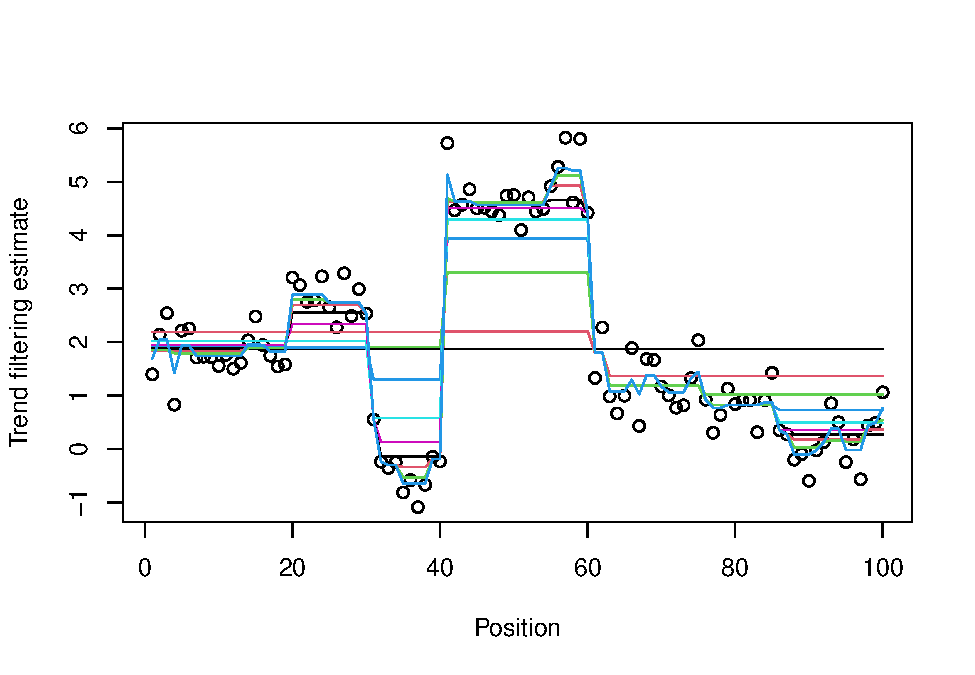
\includegraphics{High-Dimensional-Data-assignments_files/figure-latex/unnamed-chunk-33-1.pdf}

We note that the plot here is very different from the earlier examples, due to the difference in the nature of the problems (and also the packages used).

\begin{Shaded}
\begin{Highlighting}[]
\CommentTok{# Cross-validation for fused lasso; 'k' is  the}
\CommentTok{# cross-validation parameter corresponding to 'nfolds' in}
\CommentTok{# earlier cases. Cross-validation is done using the}
\CommentTok{# 'cv.trendfilter' function.}
\NormalTok{cv_fit_fused =}\StringTok{ }\KeywordTok{cv.trendfilter}\NormalTok{(fit_fused, }\DataTypeTok{k =} \DecValTok{10}\NormalTok{)}
\end{Highlighting}
\end{Shaded}

\begin{Shaded}
\begin{Highlighting}[]
\CommentTok{# Plotting the mean-squared error for different values of}
\CommentTok{# lambda in the fused lasso cross-validation}
\KeywordTok{plot}\NormalTok{(cv_fit_fused)}
\end{Highlighting}
\end{Shaded}

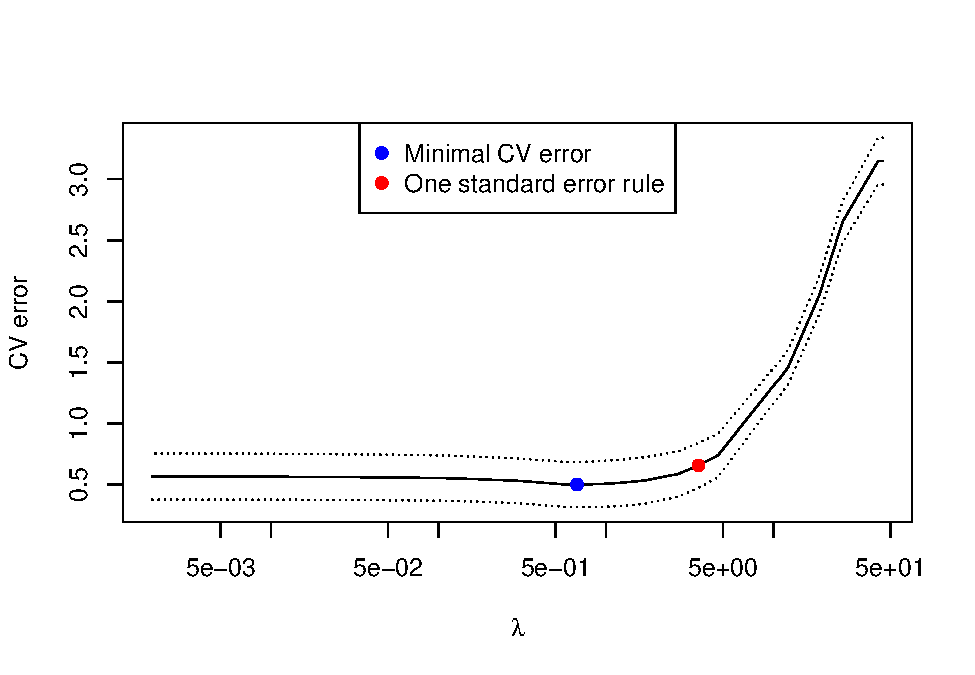
\includegraphics{High-Dimensional-Data-assignments_files/figure-latex/unnamed-chunk-35-1.pdf}

\begin{Shaded}
\begin{Highlighting}[]
\CommentTok{# Getting the lambda value corresponding to the minimum}
\CommentTok{# cross-validated error in the fused lasso}
\NormalTok{lambda_min_fused =}\StringTok{ }\NormalTok{cv_fit_fused}\OperatorTok{$}\NormalTok{lambda.min}
\KeywordTok{writeLines}\NormalTok{(}\KeywordTok{paste}\NormalTok{(}\StringTok{'Cross-validated lambda for fused lasso:'}\NormalTok{,}
\NormalTok{                 lambda_min_fused))}
\end{Highlighting}
\end{Shaded}

\begin{verbatim}
## Cross-validated lambda for fused lasso: 0.67106063258858
\end{verbatim}

\begin{Shaded}
\begin{Highlighting}[]
\CommentTok{# Plotting the fused lasso estimate for the}
\CommentTok{# cross-validated lambda along with the actual observations}
\KeywordTok{plot}\NormalTok{(fit_fused, }\DataTypeTok{lambda =}\NormalTok{ lambda_min_fused,}
     \DataTypeTok{main =} \KeywordTok{paste}\NormalTok{(}\StringTok{'Estimated coefficients for the'}\NormalTok{,}
                  \StringTok{'cross-validated lambda'}\NormalTok{))}
\end{Highlighting}
\end{Shaded}

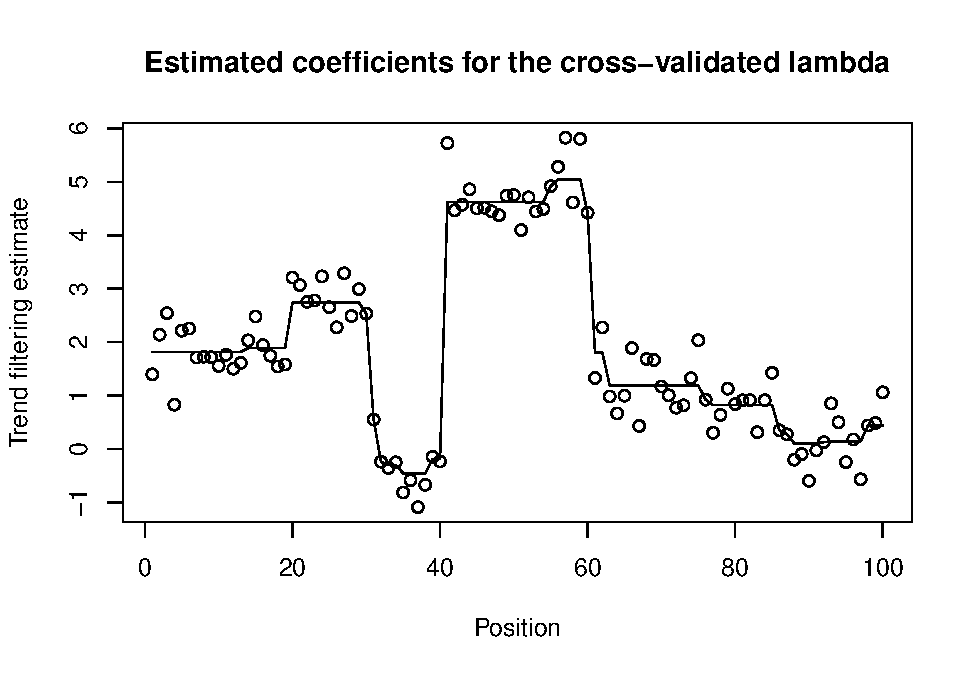
\includegraphics{High-Dimensional-Data-assignments_files/figure-latex/unnamed-chunk-35-2.pdf}

\hypertarget{multipletesting}{%
\chapter{Multiple testing}\label{multipletesting}}

In many situations, we face with the problem of conducting a collection of statistical tests simultaneously based on the same experiment. Consider the following problems:

\begin{enumerate}
\def\labelenumi{\arabic{enumi}.}
\item
  A researcher is investigating which genes make one individual susceptible to a particular disease, say, a cancer. To investigate that, data on \href{https://en.wikipedia.org/wiki/Gene_expression\#Measurement}{gene expression levels} are collected over 10000 genes from 100 normal individuals and 100 patients. The culprit genes making one susceptible to the particular disease can be discovered by finding the genes whose expression level differ significantly between a normal individual and a patient. Consequently, the researcher faces a problem of conducting 10000 statistical tests simultaneously based on a sample of 200. Such problems are common in \href{https://en.wikipedia.org/wiki/Genetic_association}{genetic association} studies.
\item
  A pharmaceutical company considers a new drug for the treatment of a particular disease, and proceeds to investigate its efficacy. Tearment of a disease often consists of alleviating of its symptoms, which can be many. So, the company is faced with conducting a \href{https://en.wikipedia.org/wiki/Randomized_controlled_trial}{randomized controlled trial} on patients, administering on group placebo and the other the experimental drug, and then conducting statistical tests to identify significant differences between the experimental group undergoing the treatment and the control group for each of the plethora of symptoms.
\end{enumerate}

In genetic studies as described in the first example, subseaquent investigation is carried out for each of the genes discovered to have a significant effect. Often, the actual number of genes associated with a disease does not exceed a few dozens. If that is the case here, and still one carries out usual hypothesis testing at 5\% level for each of the 10000 genes, it is expected that the researcher will get nearly \((10000 \times 0.05) = 500\) \emph{false positives}, which are genes that are incorrectly identified as having a significant association with the disease. This is far higher than the number of actual genes influencing the susceptibility to the disease, which means significant resources lost in further investigation in all these false positive genes.

In the second example, suppose the new drug is no better than the placebo or no intervention. However, if there are 20-30 symptoms and usual statistical tests are carried out for each of these at 5\% level, it is very probable that the new drug is found to have a significant effect for at least one syndrom.

The above examples demonstrate the limitation of usual methods of hypothesis testing while considering a family of hypotheses simultaneously for an experiment. We state the problem formally below.

Suppose we want to test \(m\) hypotheses \(H_1, \ldots, H_m\) simultaneously for an experiment, and \(m_0\) of these are actually true. Let \(R\) be the number of hypotheses rejected. The following table describes the different variables on which we shall concentrate further.

\begin{longtable}[]{@{}lccc@{}}
\caption{\label{tab:multipletesting} Classification of outcomes in multiple testing}\tabularnewline
\toprule
\begin{minipage}[b]{0.31\columnwidth}\raggedright
\strut
\end{minipage} & \begin{minipage}[b]{0.24\columnwidth}\centering
Null hypothesis is true\strut
\end{minipage} & \begin{minipage}[b]{0.25\columnwidth}\centering
Null hypothesis is false\strut
\end{minipage} & \begin{minipage}[b]{0.08\columnwidth}\centering
Total\strut
\end{minipage}\tabularnewline
\midrule
\endfirsthead
\toprule
\begin{minipage}[b]{0.31\columnwidth}\raggedright
\strut
\end{minipage} & \begin{minipage}[b]{0.24\columnwidth}\centering
Null hypothesis is true\strut
\end{minipage} & \begin{minipage}[b]{0.25\columnwidth}\centering
Null hypothesis is false\strut
\end{minipage} & \begin{minipage}[b]{0.08\columnwidth}\centering
Total\strut
\end{minipage}\tabularnewline
\midrule
\endhead
\begin{minipage}[t]{0.31\columnwidth}\raggedright
Fails to reject null hypothesis\strut
\end{minipage} & \begin{minipage}[t]{0.24\columnwidth}\centering
\(U\)\strut
\end{minipage} & \begin{minipage}[t]{0.25\columnwidth}\centering
\(W\)\strut
\end{minipage} & \begin{minipage}[t]{0.08\columnwidth}\centering
\(m - R\)\strut
\end{minipage}\tabularnewline
\begin{minipage}[t]{0.31\columnwidth}\raggedright
Rejects null hypothesis\strut
\end{minipage} & \begin{minipage}[t]{0.24\columnwidth}\centering
\(V\)\strut
\end{minipage} & \begin{minipage}[t]{0.25\columnwidth}\centering
\(S\)\strut
\end{minipage} & \begin{minipage}[t]{0.08\columnwidth}\centering
\(R\)\strut
\end{minipage}\tabularnewline
\begin{minipage}[t]{0.31\columnwidth}\raggedright
Total\strut
\end{minipage} & \begin{minipage}[t]{0.24\columnwidth}\centering
\(m_0\)\strut
\end{minipage} & \begin{minipage}[t]{0.25\columnwidth}\centering
\(m - m_0\)\strut
\end{minipage} & \begin{minipage}[t]{0.08\columnwidth}\centering
\(m\)\strut
\end{minipage}\tabularnewline
\bottomrule
\end{longtable}

Of the elements in the above table, \(R\) is the only observable variable. \(R\) is the total number of \emph{discoveries}. \(S\) is the number of \emph{true positives} (also called true discoveries), while \(V\) is the number of \emph{false positives} (also called false discoveries). In situations like the one described in the second example, one would like to bound the probability of \(V \ge 1\) (because, for example, rejection of even one hypothesis means accepting the new drug as better than placebo). The quantity \(P[ V \ge 1 ]\) is called the \emph{familywise error rate} (\textbf{FWER}).

\hypertarget{FWER}{%
\section{Controlling the familywise error rate}\label{FWER}}

Since \(P[ V \ge 1 ]\) is the probability of rejecting at least one true null hypothesis, by ensuring \(P[ V \ge 1 ] \le \alpha\), we bound the maximum familywise error rate by \(\alpha\). Below, several methods to achieve this are described.

\hypertarget{bonferroni}{%
\subsection{Bonferroni correction}\label{bonferroni}}

Suppose the level of each of the \(m\) hypotheses \(H_1, \ldots, H_m\) is \(\beta\). From the \href{https://en.wikipedia.org/wiki/Boole\%27s_inequality}{Boole's inequality}, we have \(P[ V \ge 1 ] = P\left[ \cup_{i=1}^{m} \{H_i \text{ is rejected while being true}\} \right] \le \sum_{i=1}^{m} P[H_i \text{ is rejected while being true}] = m \beta\). Therefore, to ensure FWER \(\le \alpha\), we take the level of each of the individual hypotheses as \(\alpha / m\).

The Bonferroni correction is very conservative in nature (has a high type II error), as the level of each of the individual tests is very low for even moderate \(p\). Also, when the test statistics for the hypotheses are not independent, which is often the case for high dimensional setup, the actual FWER corresponding to the Bonferroni correction is considerably lower than \(\alpha\). This can be understood from the fact that \(P[A \cup B] = P[A] + P[B] - P[A \cap B]\), which implies that for \(A\), \(B\) being dependent events, \(P[A \cup B] < P[A] + P[B]\).

Several methods were developed subsequently to mitigate the conservative nature of the Bonferroni correction. These are based on the principle of rejecting the hypotheses with the lowest p-values only, and accepting the rest.

\hypertarget{holm}{%
\subsection{Holm's method}\label{holm}}

The Holm's method, developed by \citet{holm1979simple}, first orders the p-values \(P_1, \ldots, P_m\) corresponding to the \(m\) hypotheses \(H_1, \ldots, H_m\) in the increasing order. Let the ordered p-values be \(P_{(1)}, \ldots, P_{(m)}\), and the corresponding hypotheses be \(H_{(1)}, \ldots, H_{(m)}\). For a given level \(\alpha\), let \(k\) be the smallest integer such that \[P_{(k)} > \frac{\alpha}{m - k + 1}.\] The Holm's method rejects the hypotheses \(H_{(1)}, \ldots, H_{(k-1)}\), and does not reject \(H_{(k)}, \ldots, H_{(m)}\). If \(k = 1\), it does not reject any null hypotheses, and if no such \(k\) exists, it rejects all the null hypotheses.

It is easy to see that, whenever the Bonferroni correction rejects a particular hypothesis, the Holm's method also rejects it, but not the contrary. It can be proved that FWER \(\le \alpha\) for the Holm's method. Hence, the Holm's method is uniformly more powerful than the Bonferroni correction.

\hypertarget{hochberg}{%
\subsection{Hochberg's method}\label{hochberg}}

Hochberg's method \citep{hochberg1988sharper} also orders the p-values in the increasing order as in \ref{holm}. However, it finds the largest integer \(k\) such that \[P_{(k)} \le \frac{\alpha}{m - k + 1},\] and then rejects \(H_{(1)}, \ldots, H_{(k)}\) but does not reject \(H_{(k+1)}, \ldots, H_{(m)}\).

At the first glance, the Holm's method and the Hochberg's method may seem identical, but in fact Hochberg's method is uniformly more powerful than the former. This is due to the fact that the Hochberg's method rejects \(H_{(1)}, \ldots, H_{(k)}\) whenever the Holm's method rejects them, but not the other way. Intuitively, because the Hochberg's method considers the p-values from the highest to the lowest, it is always inclined to reject more hypotheses than the Holm's method.
However, unlike the Holm's method, whose bound on FWER does not need any assumption on the underlying distribution or dependence among the p-values or test statistics, the Hochberg's method does (\citet{sarkar1997simes}, \citet{sarkar1998some}). Its bound on FWER is valid in particular when the test statistics for the individual hupotheses are indepdendent or positively correlated.

\hypertarget{hommel}{%
\subsection{Hommel's method}\label{hommel}}

In the Hommel's method \citep{hommel1988stagewise}, one again orders the p-values as in \ref{holm}, then finds the maximum integer \(j\) in \(1, \ldots, n\) such that \[P_{(n - j + k)} > \frac{k \alpha}{j}\] for all \(k = 1, \ldots, j\). If such a maximum \(j\) does not exist, one rejects all the null hypotheses \(H_i\), \(i = 1, \ldots, m\). Otherwise, one rejects the hypotheses whose corresponding p-values satisfy \(P_i \le \alpha / j\).

It can be shown that the Hommel's method is more powerful than the Hochberg's method. However, the validity of the bound on its FWER also requires certain assumptions.

\hypertarget{FDR}{%
\section{False discovery rate and its control}\label{FDR}}

In certain situations, it may not be appropriate to put a bound on the FWER. Consider the example of the gene expression experiment described in the beginning of Chapter \ref{multipletesting}. If there are, say, 30 genes with actual effect on the disease, and in the testing 2 false positives occur, then it is not a very significant problem in terms of drawing wrong conclusions and wastage of resources. Similarly, if there are 200 genes affecting the disease in reality, and we have 20 false positives, then again it is not a big issue. In such cases, controlling the FWER makes the statistical investigation too conservative for the present purpose, and a certain kind of adaptablity in the procedure is desired based on the number of true positives. In such cases, we want to control the number of false positives compared to the true positives, as opposed to the occurance of any false positives.

Consider the quantities described in Table \ref{tab:multipletesting}. Recall that the variable \(R\) denotes the number of rejected null hypotheses (discoveries) and \(V\) is the number of rejected true hypotheses (false discoveries). We want to put a bound on the expected value of the ratio \((V / R)\). The quantity \((V / R)\) is called the \emph{false discovery proportion}, and \(E[ V / R ]\) is called the \emph{false discovery rate} (\textbf{FDR}). We assume the convention of defining \(0 / 0 = 0\). Below, two methods are described which control the FDR.

\hypertarget{BH}{%
\subsection{Benjamini-Hochberg method}\label{BH}}

The Benjamini-Hochberg method \citep{benjamini1995controlling} finds the largest integer \(k\) such that \[P_{(k)} \le \frac{\alpha}{m} k\] for a given level \(\alpha\). It then rejects all \(H_{(i)}\) for \(i = 1, \ldots, k\).

This method can be represented by a plot of the ordered p-values along with a line passing through the origin having slope \((\alpha / m)\). The hypotheses, whose corresponding p-values are below the line, are rejected.

It can be shown that this method has a FDR less than or equal to \alpha when the test statistics are independent, and under certain depdendence conditions. However, this is not valid for arbitrary dependence structures.

\hypertarget{BY}{%
\subsection{Benjamini--Yekutieli method}\label{BY}}

The Benjamini--Yekutieli method \citep{benjamini2001control} modifies the Benjamini-Hochberg method so that it controls the FDR under general dependene structures. This method finds the largest \(k\) such that \[P_{(k)} \le \frac{\alpha}{m h(m)} k ,\] where \(h(m) = \sum_{i=1}^m \frac{1}{i}\), and then rejects all \(H_{(i)}\) for \(i = 1, \ldots, k\). However, if the test statistics are independent or the dependence conditions in the Benjamini-Hochberg method are satisfied, one can take \(h(m) = 1\).

The FDR of the Benjamini--Yekutieli method is bounded above by \(\alpha\), as indicated earlier.

\hypertarget{adjusted-pvalues}{%
\section{Adjusted p-values}\label{adjusted-pvalues}}

In hypothesis testing, we are often more interested in the p-value of the test instead of accepting or rejecting the null hypothesis at some specified level. Reporting the p-value only makes our inference independent of the level of the test. In multiple testing, we have seen that the methods are designed to reject or not reject the individual hypotheses based on their p-values and a pre-specified level. Nevertheless, for each of the methods described above, one can modify the p-values obtained for the individual hypothesis so that one can follow the usual procedure of hypothesis testing based on those modified p-values and any level and still control the FWER or FDR as intended. These modified p-values are called \emph{adjusted p-values}. The adjusted p-values are numbers lying in the interval {[}0, 1{]}, but they should not be interpreted as some probabilities like actual p-values.

\begin{itemize}
\item
  In the Bonferroni correction (\ref{bonferroni}), one rejects hypothesis \(H_i\) at level \(\alpha\) if the corresponding p-value \(P_i\) satisfies \(P_i \le \alpha / m\). Therefore the adjusted p-value \(\hat{P}_i\) for hypothesis \(H_i\) for the Bonferroni correction is \(\hat{P}_i = \min\{ m P_i, 1 \}\), \(i = 1, \ldots, m\). The minimum with 1 is taken to bound the p-value in the interval \([0, 1]\).
\item
  The adjusted p-values for the Holm's method (\ref{holm}) are given by \(\hat{P}_{(i)} = \min\left\{ \max\{ (m + 1 - j) P_{(j)} \,|\, j = 1, \ldots, i \}, 1 \right\}\), \(i = 1, \ldots, m\). (Multiplication by \((m + 1 - j)\) is obvious. Why the cumulative maximum is taken? Convince yourself that it is needed.)
\item
  The adjusted p-values for the Hochberg's method (\ref{hochberg}) are given by \(\hat{P}_{(i)} = \min\left\{ \min\{ (m + 1 - j) P_{(j)} \,|\, j = i, \ldots, m \}, 1 \right\}\), \(i = 1, \ldots, m\). Note that, though the difference in the descriptions of the Holm's method and the Hochberg's method may not be obvious initially, the formulae for their adjusted p-values are clearly distinct.
\item
  Calculation of the adjusted p-values for the Hommel's method (\ref{hommel}) is relatively complicated. These are computed algorithmically (given by \citet{wright1992adjusted}), unlike the straightforward formulae for the other methods.
\item
  The adjusted p-values for the Benjamini-Hochberg method (\ref{BH}) are given by \(\hat{P}_{(i)} = \min\left\{ \min\left\{ \frac{m}{j} P_{(j)} \,\middle|\, j = i, \ldots, m \right\}, 1 \right\}\), \(i = 1, \ldots, m\).
\item
  The adjusted p-values for the Benjamini--Yekutieli method (\ref{BY}) are given by \(\hat{P}_{(i)} = \min\left\{ \min\left\{ \frac{m h(m)}{j} P_{(j)} \,\middle|\, j = i, \ldots, m \right\}, 1 \right\}\), \(i = 1, \ldots, m\), where \(h(m) = \sum_{j=1}^m \frac{1}{j}\).
\end{itemize}

\hypertarget{multipletesting-summary}{%
\section{Summary}\label{multipletesting-summary}}

While testing simultaneously many hypotheses, one may be interested in controlling the probability of rejecting atleast one true null hypothesis (FWER) or the expected proportion of rejected true null hypotheses (FDR). There are several methods to achieve either one. The Bonferroni correction, the Holm's method, the Hochberg's method and the Hommel's method control the FWER. The Benjamini-Hochberg method and the Benjamini--Yekutieli method control the FDR.

All the methods described in this chapter make very broad assumptions about the dependence among the test statistics for the individual tests (or does not make any assumption about dependence; for example: the Bonferroni correction). As a consequence, these are relatively conservative procedures, and it is possible to develop methods which are more powerful than them by taking into account the dependence structure of the test statistics in the particular multiple testing scenario. Resampling based methods (bootstrap and permutation) are develop with this aim, and they generally are more powerful than the methods described before. Those are out of scope of the present document.

\hypertarget{multipletesting-demonstration}{%
\section{Numerical demonstration}\label{multipletesting-demonstration}}

All the methods for adjusted p-value computation described in \ref{adjusted-pvalues} are implemented in the function \texttt{p.adjust} available in the R package \textbf{stats} (included with base R distribution). Below, the use of this function is demonstrated.

Consider a simple case where we have 10 hypotheses each having a p-value 0.04. What will be the adjusted p-values for the various methods described in sections \ref{FWER} and \ref{FDR}? Their computation is presented below.

\begin{Shaded}
\begin{Highlighting}[]
\CommentTok{# Vector of p-values with length 10 and each element being 0.04}
\NormalTok{p =}\StringTok{ }\KeywordTok{rep}\NormalTok{(}\FloatTok{0.04}\NormalTok{, }\DecValTok{10}\NormalTok{)}
\KeywordTok{writeLines}\NormalTok{(}\KeywordTok{paste}\NormalTok{(}\StringTok{'Actual p-values:}\CharTok{\textbackslash{}n}\StringTok{'}\NormalTok{, }\KeywordTok{paste}\NormalTok{(p, }\DataTypeTok{collapse =} \StringTok{' '}\NormalTok{)))}

\CommentTok{# Bonferroni correction}
\NormalTok{p_bonferroni =}\StringTok{ }\KeywordTok{p.adjust}\NormalTok{(p, }\DataTypeTok{method =} \StringTok{'bonferroni'}\NormalTok{)}
\KeywordTok{writeLines}\NormalTok{(}\KeywordTok{paste}\NormalTok{(}\StringTok{'Adjusted p-values for the'}\NormalTok{,}
                 \StringTok{'Bonferroni correction:}\CharTok{\textbackslash{}n}\StringTok{'}\NormalTok{,}
                 \KeywordTok{paste}\NormalTok{(p_bonferroni, }\DataTypeTok{collapse =} \StringTok{' '}\NormalTok{)))}

\CommentTok{# Holm's method}
\NormalTok{p_holm =}\StringTok{ }\KeywordTok{p.adjust}\NormalTok{(p, }\DataTypeTok{method =} \StringTok{'holm'}\NormalTok{)}
\KeywordTok{writeLines}\NormalTok{(}\KeywordTok{paste}\NormalTok{(}\StringTok{'Adjusted p-values for the'}\NormalTok{,}
                 \StringTok{'Holm}\CharTok{\textbackslash{}'}\StringTok{s method:}\CharTok{\textbackslash{}n}\StringTok{'}\NormalTok{,}
                 \KeywordTok{paste}\NormalTok{(p_holm, }\DataTypeTok{collapse =} \StringTok{' '}\NormalTok{)))}

\CommentTok{# Hochberg's method}
\NormalTok{p_hochberg =}\StringTok{ }\KeywordTok{p.adjust}\NormalTok{(p, }\DataTypeTok{method =} \StringTok{'hochberg'}\NormalTok{)}
\KeywordTok{writeLines}\NormalTok{(}\KeywordTok{paste}\NormalTok{(}\StringTok{'Adjusted p-values for the'}\NormalTok{,}
                 \StringTok{'Hochberg}\CharTok{\textbackslash{}'}\StringTok{s method:}\CharTok{\textbackslash{}n}\StringTok{'}\NormalTok{,}
                 \KeywordTok{paste}\NormalTok{(p_hochberg, }\DataTypeTok{collapse =} \StringTok{' '}\NormalTok{)))}

\CommentTok{# Hommel's method}
\NormalTok{p_hommel =}\StringTok{ }\KeywordTok{p.adjust}\NormalTok{(p, }\DataTypeTok{method =} \StringTok{'hommel'}\NormalTok{)}
\KeywordTok{writeLines}\NormalTok{(}\KeywordTok{paste}\NormalTok{(}\StringTok{'Adjusted p-values for the'}\NormalTok{,}
                 \StringTok{'Hommel}\CharTok{\textbackslash{}'}\StringTok{s method:}\CharTok{\textbackslash{}n}\StringTok{'}\NormalTok{,}
                 \KeywordTok{paste}\NormalTok{(p_hommel, }\DataTypeTok{collapse =} \StringTok{' '}\NormalTok{)))}

\CommentTok{# Benjamini-Hochberg method}
\NormalTok{p_BH =}\StringTok{ }\KeywordTok{p.adjust}\NormalTok{(p, }\DataTypeTok{method =} \StringTok{'BH'}\NormalTok{)}
\KeywordTok{writeLines}\NormalTok{(}\KeywordTok{paste}\NormalTok{(}\StringTok{'Adjusted p-values for the'}\NormalTok{,}
                 \StringTok{'Benjamini-Hochberg method:}\CharTok{\textbackslash{}n}\StringTok{'}\NormalTok{,}
                 \KeywordTok{paste}\NormalTok{(p_BH, }\DataTypeTok{collapse =} \StringTok{' '}\NormalTok{)))}

\CommentTok{# Benjamini–Yekutieli method}
\NormalTok{p_BY =}\StringTok{ }\KeywordTok{p.adjust}\NormalTok{(p, }\DataTypeTok{method =} \StringTok{'BY'}\NormalTok{)}
\KeywordTok{writeLines}\NormalTok{(}\KeywordTok{paste}\NormalTok{(}\StringTok{'Adjusted p-values for the'}\NormalTok{,}
                 \StringTok{'Benjamini–Yekutieli method:}\CharTok{\textbackslash{}n}\StringTok{'}\NormalTok{,}
                 \KeywordTok{paste}\NormalTok{(}\KeywordTok{round}\NormalTok{(p_BY, }\DecValTok{3}\NormalTok{), }\DataTypeTok{collapse =} \StringTok{' '}\NormalTok{)))}
\end{Highlighting}
\end{Shaded}

\begin{verbatim}
## Actual p-values:
##  0.04 0.04 0.04 0.04 0.04 0.04 0.04 0.04 0.04 0.04
## Adjusted p-values for the Bonferroni correction:
##  0.4 0.4 0.4 0.4 0.4 0.4 0.4 0.4 0.4 0.4
## Adjusted p-values for the Holm's method:
##  0.4 0.4 0.4 0.4 0.4 0.4 0.4 0.4 0.4 0.4
## Adjusted p-values for the Hochberg's method:
##  0.04 0.04 0.04 0.04 0.04 0.04 0.04 0.04 0.04 0.04
## Adjusted p-values for the Hommel's method:
##  0.04 0.04 0.04 0.04 0.04 0.04 0.04 0.04 0.04 0.04
## Adjusted p-values for the Benjamini-Hochberg method:
##  0.04 0.04 0.04 0.04 0.04 0.04 0.04 0.04 0.04 0.04
## Adjusted p-values for the Benjamini–Yekutieli method:
##  0.117 0.117 0.117 0.117 0.117 0.117 0.117 0.117 0.117 0.117
\end{verbatim}

From the output above, the difference between the adjusted p-values of the Holm's method and the Hochberg's method is noticeable. It corroborates our earlier assertion in subsection \ref{hochberg} that the Hochberg's method is uniformly more powerful than the Holm's method, as every adjusted p-value for the Hochberg's method is smaller than the corresponding adjusted p-value for the Holm's method. However, though the Holm's method is uniformly more powerfull than the Bonferroni correction and the Hommel method is more powerful than the Hochberg's method, this toy example cannot confirm them, as all the corresponding adjusted p-values are identical. If we conduct simultaneous testing at level 0.05, the Bonferroni correction, the Holm's method and the Benjamini--Yekutieli method fail to reject any hothesis, whereas the Hochberg's method, the Hommel's method and the Benjamini-Hochberg method reject all the hypotheses.

Next, we consider a real dataset: the \texttt{golub} dataset from the R package \textbf{multtest} available in \href{https://www.bioconductor.org/packages/release/bioc/html/multtest.html}{Bioconductor}. This dataset contains the expression levels of 3051 genes based on 38 tumor mRNA samples from a leukemia microarray study presented in \citet{golub1999molecular}. Among the 38 tumor samples, 27 are acute lymphoblastic leukemia (ALL) cases and 11 are acute myeloid leukemia (AML) cases. The \texttt{golub} datatset is a matrix with 3051 rows and 38 columns. Each row corresponds to a gene, the first 27 columns correspond to ALL cases and the last 11 columns correspond to AML cases. We are interested in investigating the presence of statistically significant differences in expression levels for the 3051 genes among the two types of cancers.

First we need to install the `multtest' package from Bioconductor, which can be done using the function `install' from the package `BiocManager'. The code in the next line would do this.

\begin{Shaded}
\begin{Highlighting}[]
\NormalTok{BiocManager}\OperatorTok{::}\KeywordTok{install}\NormalTok{(}\StringTok{'multtest'}\NormalTok{)}
\end{Highlighting}
\end{Shaded}

Now, the computation procedure is demonstrated below.

\begin{Shaded}
\begin{Highlighting}[]
\CommentTok{# Loading the data from the package 'multtest'}
\KeywordTok{data}\NormalTok{(}\StringTok{'golub'}\NormalTok{, }\DataTypeTok{package =} \StringTok{'multtest'}\NormalTok{)}

\CommentTok{# Storing the data corresponding to ALL cases in the}
\CommentTok{# variable golub_ALL}
\NormalTok{golub_ALL =}\StringTok{ }\NormalTok{golub[,}\DecValTok{1}\OperatorTok{:}\DecValTok{27}\NormalTok{]}

\CommentTok{# Storing the data corresponding to AML cases in the}
\CommentTok{# variable golub_AML}
\NormalTok{golub_AML =}\StringTok{ }\NormalTok{golub[,}\DecValTok{28}\OperatorTok{:}\DecValTok{38}\NormalTok{]}

\CommentTok{# m is the number of tests, which is equal to the}
\CommentTok{# number of genes}
\NormalTok{m =}\StringTok{ }\KeywordTok{nrow}\NormalTok{(golub)}

\CommentTok{# Computing the p-values using a two-sample t test}
\NormalTok{p =}\StringTok{ }\KeywordTok{c}\NormalTok{()}
\ControlFlowTok{for}\NormalTok{ (i }\ControlFlowTok{in} \DecValTok{1}\OperatorTok{:}\NormalTok{m)}
\NormalTok{  p[i] =}\StringTok{ }\KeywordTok{t.test}\NormalTok{(golub_ALL[i,], golub_AML[i,],}
                \DataTypeTok{alternative =} \StringTok{'two.sided'}\NormalTok{)}\OperatorTok{$}\NormalTok{p.value}

\CommentTok{# Calculating the adjusted p-values}
\NormalTok{p_bonferroni =}\StringTok{ }\KeywordTok{p.adjust}\NormalTok{(p, }\DataTypeTok{method =} \StringTok{'bonferroni'}\NormalTok{)}
\NormalTok{p_holm =}\StringTok{ }\KeywordTok{p.adjust}\NormalTok{(p, }\DataTypeTok{method =} \StringTok{'holm'}\NormalTok{)}
\NormalTok{p_hochberg =}\StringTok{ }\KeywordTok{p.adjust}\NormalTok{(p, }\DataTypeTok{method =} \StringTok{'hochberg'}\NormalTok{)}
\NormalTok{p_hommel =}\StringTok{ }\KeywordTok{p.adjust}\NormalTok{(p, }\DataTypeTok{method =} \StringTok{'hommel'}\NormalTok{)}
\NormalTok{p_BH =}\StringTok{ }\KeywordTok{p.adjust}\NormalTok{(p, }\DataTypeTok{method =} \StringTok{'BH'}\NormalTok{)}
\NormalTok{p_BY =}\StringTok{ }\KeywordTok{p.adjust}\NormalTok{(p, }\DataTypeTok{method =} \StringTok{'BY'}\NormalTok{)}

\CommentTok{# Calculating the number of rejections based on level 0.05.}
\NormalTok{alpha =}\StringTok{ }\FloatTok{0.05}
\KeywordTok{writeLines}\NormalTok{(}\KeywordTok{paste}\NormalTok{(}\StringTok{'Number of rejections based on'}\NormalTok{,}
                 \StringTok{'unadjusted p-values:'}\NormalTok{, }\KeywordTok{sum}\NormalTok{(p }\OperatorTok{<=}\StringTok{ }\NormalTok{alpha)))}
\KeywordTok{writeLines}\NormalTok{(}\KeywordTok{paste}\NormalTok{(}\StringTok{'Number of rejections based on'}\NormalTok{,}
                 \StringTok{'Bonferroni correction:'}\NormalTok{,}
                 \KeywordTok{sum}\NormalTok{(p_bonferroni }\OperatorTok{<=}\StringTok{ }\NormalTok{alpha)))}
\KeywordTok{writeLines}\NormalTok{(}\KeywordTok{paste}\NormalTok{(}\StringTok{'Number of rejections based on'}\NormalTok{,}
                 \StringTok{'Holm}\CharTok{\textbackslash{}'}\StringTok{s method:'}\NormalTok{,}
                 \KeywordTok{sum}\NormalTok{(p_holm }\OperatorTok{<=}\StringTok{ }\NormalTok{alpha)))}
\KeywordTok{writeLines}\NormalTok{(}\KeywordTok{paste}\NormalTok{(}\StringTok{'Number of rejections based on'}\NormalTok{,}
                 \StringTok{'Hochberg}\CharTok{\textbackslash{}'}\StringTok{s method:'}\NormalTok{,}
                 \KeywordTok{sum}\NormalTok{(p_hochberg }\OperatorTok{<=}\StringTok{ }\NormalTok{alpha)))}
\KeywordTok{writeLines}\NormalTok{(}\KeywordTok{paste}\NormalTok{(}\StringTok{'Number of rejections based on'}\NormalTok{,}
                 \StringTok{'Hommel}\CharTok{\textbackslash{}'}\StringTok{s method:'}\NormalTok{,}
                 \KeywordTok{sum}\NormalTok{(p_hommel }\OperatorTok{<=}\StringTok{ }\NormalTok{alpha)))}
\KeywordTok{writeLines}\NormalTok{(}\KeywordTok{paste}\NormalTok{(}\StringTok{'Number of rejections based on'}\NormalTok{,}
                 \StringTok{'Benjamini-Hochberg method:'}\NormalTok{,}
                 \KeywordTok{sum}\NormalTok{(p_BH }\OperatorTok{<=}\StringTok{ }\NormalTok{alpha)))}
\KeywordTok{writeLines}\NormalTok{(}\KeywordTok{paste}\NormalTok{(}\StringTok{'Number of rejections based on'}\NormalTok{,}
                 \StringTok{'Benjamini–Yekutieli method:'}\NormalTok{,}
                 \KeywordTok{sum}\NormalTok{(p_BY }\OperatorTok{<=}\StringTok{ }\NormalTok{alpha)))}
\end{Highlighting}
\end{Shaded}

\begin{verbatim}
## Number of rejections based on unadjusted p-values: 1078
## Number of rejections based on Bonferroni correction: 103
## Number of rejections based on Holm's method: 103
## Number of rejections based on Hochberg's method: 103
## Number of rejections based on Hommel's method: 108
## Number of rejections based on Benjamini-Hochberg method: 695
## Number of rejections based on Benjamini–Yekutieli method: 293
\end{verbatim}

We note that the Bonferroni's correction is the most conservative procedure, as expected. However, here the Holm's method and the Hochberg's method are also as much conservative as the Bonferroni's correction. The FDR controlling procedures are relatively less conservative compared to the FWER controlling procedures, again as expected.

\hypertarget{assignments}{%
\chapter{Assignments}\label{assignments}}

\begin{enumerate}
\def\labelenumi{\arabic{enumi}.}
\item
  Fix your roll number as the seed. Let \(\Sigma\) be a \(80 \times 80\) covariance matrix defined by \(\sigma_{i j} = 0.6 + 0.6 \mathbb{I}(i = j)\). Let \(X\) be a \(80\) dimensional random vector with \(X \sim N_{80}( 0, \Sigma )\). Denote the \(i\)th coordinate of \(X\) as \(X_i\), \(i = 1, \ldots, 80\). Consider the following regression problem: \(Y = (1 + X_1 + 2 X_2 - 3 X_3 - 4 X_4 + 5 X_5) + e\), where \(e\) is an error variable independent of \(X\). Generate a sample of size \(30\) on \(Y\) and \(X\). Generate also a sample of size 5 from the distribution of \(X\), and name the data matrix as \(X_0\). Based on this sample,

  \begin{itemize}
  \item
    Compute and plot the lasso solution paths.
  \item
    Compute and visually present the outputs of the cross-validation process for the tuning parameter \(\lambda\).
  \item
    Print the value of \(\lambda\) giving the minimum cross-validated error.
  \item
    Print the value of \(\lambda\) giving the most regularized model such that its cross-validated error is within one standard error of the minimum.
  \item
    Print the estimated coefficients of the fitted lasso model for the value \(\lambda\) being the one giving the minimum cross-validated error.
  \item
    Print the estimated coefficients of the fitted lasso model for \(\lambda = 0.5\).
  \item
    Print the number of nonzero coefficients for the value \(\lambda\) being the one giving the minimum cross-validated error.
  \item
    Predict the response values at the covariate values in \(X_0\) for \(\lambda\) being the minimizer of the cross-validated error.
  \end{itemize}
\item
  Based on the same data as above, solve all the above problems for the ridge regression method.
\item
  Again, based on the same data as above, solve all the above problems for the elastic net method, taking \(\alpha = 0.5\).
\item
  Generate an independent sample of size \(1000\) from the \(Beta(1, 100)\) distribution, and assume that they are the p-values of \(1000\) hypotheses tested simultaneously.

  \begin{itemize}
  \item
    Compute the corresponding adjusted p-values for the Bonferroni correction, the Holm's method, the Hochberg's method, the Hommel's method, the Benjamini-Hochberg method and the Benjamini--Yekutieli method.
  \item
    Compute the number of rejections in each case for the level being \(0.05\).
  \end{itemize}
\end{enumerate}

Marks: (1): 10, (2): 3, (3): 3, (4): 4

  \bibliography{references.bib,packages.bib}

\end{document}
